\documentclass[11pt]{article}

\usepackage[a4paper,margin=27mm]{geometry}
\usepackage{amsmath,amssymb,amsthm,mathtools}
\usepackage{array}
\usepackage{booktabs}
\usepackage{enumitem}
\usepackage{graphicx}
\usepackage[hidelinks]{hyperref}
\usepackage{xcolor}
\usepackage{tikz}
\usetikzlibrary{arrows.meta,positioning}
\usepackage{pgfplots}
\pgfplotsset{compat=1.18}
\usepackage{microtype}
\usepackage[T1]{fontenc}
\usepackage{lmodern}
\setlength{\emergencystretch}{2em}

\definecolor{protocolblue}{RGB}{31,78,121}
\definecolor{protocolgray}{RGB}{245,247,249}
\newcommand{\norm}[1]{\left\lVert #1\right\rVert}
\newcommand{\C}{\mathbb{C}}
\newcommand{\R}{\mathbb{R}}
\newtheorem{theorem}{Theorem}
\newtheorem{corollary}[theorem]{Corollary}
\newtheorem{proposition}[theorem]{Proposition}

\title{\textbf{Band equivalence versus hopping locality: exact rank-two geometry
and a smooth continuum benchmark}}
\author{KSD reduced-Hamiltonian research program}
\date{Theoretical and computational protocol manuscript}

\begin{document}
\maketitle

\begin{abstract}
A conventional Bloch calculation cannot distinguish matrix fields related by a
momentum-dependent unitary similarity because their bands are identical. The similarity
can nevertheless redistribute real-space hopping blocks and produce a nonzero matrix
residual when the allowed identification is restricted to one momentum-independent real
rotation. We derive the exact adequacy geometry for a rank-two candidate that shifts the
energy centroid and positively rescales the traceless level splitting. The spectral loss
and every restricted-alignment matrix loss share one diagonal quadratic curvature. Their
admissible sets are homothetic ellipses controlled by a splitting scale $\kappa$ and a
normalized correlation $\mu$. We then construct the smooth family
$U_a(q)=R(a\sin2\pi q)$. Although every member has exactly the same bands, its minimum
restricted-alignment threshold rises as $\sqrt{\kappa[1-J_0(2a)^2]}$; under exact
spectral acceptance, the joint threshold rises as
$\sqrt{2\kappa[1-J_0(2a)]}$. For a spectrally flat traceless parent, the squared
irreducible matrix residual equals the total Fourier weight in nonzero-range hopping
blocks generated by the momentum-dependent representation. A pre-version calculation
verifies these flat-parent channels under nested momentum refinement and separately
exposes unresolved amplitude interpolation. An initial non-flat four-state calculation
using the same smooth family preserves roundoff-level band agreement while redistributing
existing hopping weight. Its frame-invariant momentum controls converge, while amplitude
interpolation remains unresolved. A bounded parent-hopping homotopy shows the mechanism
throughout five sampled dispersion scales. An exploratory ordinary-lattice truncation
layer then demonstrates on a disjoint mesh that the rotated representation requires
substantially greater hopping range for comparable band accuracy.
\end{abstract}

\noindent\textbf{Keywords:} reduced Hamiltonian; model adequacy; admissible set;
periodic system; spectral error; operator error; convergence; Fourier locality

\paragraph{Experiment identity.}
The publication-independent experiment is named \emph{Band Equivalence versus Hopping
Locality}. Its family identity is
\path{ksdft2effmass.campaign.model-adequacy.periodic1d.band-equivalence-versus-hopping-locality}.

\paragraph{Scope.}
The threshold continuum and admissible-set formulas are analytic results. A pre-version
flat-parent calculation is reported in Section~\ref{sec:exploratory-analysis} as
development analysis, not as retained evidence. Section~\ref{sec:nonflat-exploratory}
reports an initial four-state execution whose parent has finite-range hopping, with
`converged' momentum refinement and `unresolved' amplitude interpolation. Complete
Fourier inventories are analyzed first; a separate exploratory action converts them to
ordinary-lattice models, applies explicit symmetric cutoffs, and reports pointwise band
consequences. Its parameter bounds, instance-specific
acceptance and separation
controls, locality ranges, and final numerical tolerances are not frozen. No retained
run or accepted instance-specific scientific disposition is asserted here. Non-flat
numerical claims are pointwise at declared amplitude nodes; plotted connections are
guides to the eye, and continuous-amplitude interpolation is treated as a separate
supplementary approximation problem.

\section{Introduction}

A reduced Hamiltonian can reproduce selected band energies while failing to reproduce
a matrix field under a declared identification of retained coordinates. The distinction
matters whenever the scientific interpretation depends on matrix elements, finite-range
hopping blocks, or locality. Eigenvalues are invariant under a basis rotation, whereas
matrix entries and Fourier hopping blocks are not. If the generating momentum-dependent
unitary is admitted as the state-space identification, the two matrix fields represent
the same abstract operator and the corresponding residual vanishes. The question here
is deliberately narrower: can one momentum-independent real rotation identify the
fields while retaining their hopping representation? Spectral agreement and this
restricted-alignment agreement are related but non-equivalent requirements.

The main question is how strongly these two notions of adequacy can diverge while the
Bloch bands remain exactly unchanged. We study a two-band candidate controlled by an
energy-centroid shift and a rescaling of the level splitting. The operator comparison
additionally allows one global real rotation of the retained basis. A one-parameter
family of momentum-dependent target rotations then produces identical bands but a
continuously increasing operator-acceptance threshold.

Three outcomes are possible. A \emph{joint match} is established by exhibiting one
parameter pair that passes both error limits. \emph{Certified separation} is established
only when a verified lower bound places the two admissible parameter regions farther
apart than a declared numerical resolution. If neither statement is established, the
outcome is \emph{unresolved}. A failed search for a joint match is not a separation
proof, and a plot or local optimizer result is not a global certificate.

The central result is an exact reduction of that decision problem. Both losses have the
same diagonal quadratic curvature, so the spectral admissible set and every aligned
matrix-loss component are homothetic ellipses. Their centers, radii, compatibility
condition, and separation distance follow from one splitting scale and one
angle-dependent correlation coefficient. For the symmetric rotation family, those
quantities yield an explicit monotone threshold curve. The completed flat-parent calculation
evaluates the analytic channels without fitting. An initial non-flat implementation
evaluates the gap, frame, harmonic, threshold, Fourier, Parseval, and reconstruction
channels, while the full admissible-set and post-decision certificate workflow remains
prospective.

The computational protocol separates three numerical roles. Construction coordinates determine the
loss quadratics, witnesses, certificates, and disposition. Nested construction meshes
determine whether those quantities have converged. A final staggered evaluation mesh is
used only after the disposition has been fixed and probes behavior between construction
nodes. This separation prevents post-decision diagnostics from changing the scientific
question that was actually tested.

\section{Finite-range periodic realization}

\subsection{Finite-range parent Hamiltonian}

The controlled parent is a one-dimensional periodic model with lattice period $a_0$ and
four states per cell. Let $k$ denote the physical Bloch wavenumber and
$G=2\pi/a_0$ the primitive reciprocal-lattice magnitude. The calculation uses the
dimensionless reduced coordinate
\begin{equation}
 q=\frac{k}{G}=\frac{k a_0}{2\pi},
 \qquad -\frac12\le q<\frac12.
 \label{eq:reduced-wavenumber}
\end{equation}
Thus $k$ has units of inverse length, whereas $q$ is expressed in reciprocal-lattice
units. The reduced coordinate is used below because lattice translations then enter as
$e^{2\pi iqR}$ with integer cell displacement $R$. The four states are grouped into a
lower two-orbital sector and an upper two-orbital sector. In
this block convention, the nonzero hopping matrices are
\begin{equation}
 T_0=
 \begin{pmatrix}
 D_{\mathrm L}&0\\
 0&D_{\mathrm U}
 \end{pmatrix},
 \qquad
 T_{+1}=
 \begin{pmatrix}
 J_{\mathrm L}&V\\
 0&J_{\mathrm U}
 \end{pmatrix},
 \qquad
 T_{-1}=T_{+1}^\dagger.
 \label{eq:parent-hopping-blocks}
\end{equation}
In units of the positive energy scale $E_G$, the $2\times2$ blocks are
\begin{align}
 D_{\mathrm L}&=
 \begin{pmatrix}-1.20&0.06\\0.06&-0.35\end{pmatrix},
 &
 D_{\mathrm U}&=
 \begin{pmatrix}1.00&0.04\\0.04&1.75\end{pmatrix},\\
 J_{\mathrm L}&=
 \begin{pmatrix}0.15&0\\0&-0.10\end{pmatrix},
 &
 J_{\mathrm U}&=
 \begin{pmatrix}0.05&0\\0&-0.04\end{pmatrix},
 &
 V&=
 \begin{pmatrix}0.12&0\\0&0.10\end{pmatrix}.
 \label{eq:parent-numerical-blocks}
\end{align}
Thus $D_{\mathrm L}$ and $D_{\mathrm U}$ describe intracell mixing within the lower and
upper sectors, $J_{\mathrm L}$ and $J_{\mathrm U}$ describe nearest-cell hopping within
each sector, and $V$ couples the lower sector in one cell to the upper sector in the
neighboring cell. Hermitian conjugation supplies the reverse coupling.

With $z=e^{2\pi iq}$, the Bloch Hamiltonian can be read directly in the same convention:
\begin{equation}
 K(q)=
 \begin{pmatrix}
 D_{\mathrm L}+zJ_{\mathrm L}+z^{-1}J_{\mathrm L}^\dagger & zV\\
 z^{-1}V^\dagger & D_{\mathrm U}+zJ_{\mathrm U}+z^{-1}J_{\mathrm U}^\dagger
 \end{pmatrix}
 =\sum_{R=-1}^{1}e^{2\pi iqR}T_R.
 \label{eq:parent-bloch}
\end{equation}
These block values define the parent Hamiltonian rather than one particular momentum
sample. All resolution levels evaluate this same parent; refinement changes only the
set of sampled momenta. The model is synthetic rather than material-specific. Its two
internally mixed orbital sectors are separated in onsite energy but coupled across
neighboring cells, producing a momentum-dependent retained subspace with finite hopping
support.

\subsection{Conventional Bloch-band solution}
\label{sec:conventional-bloch}

The analysis begins with the standard Bloch calculation. In operator notation, the
cell-periodic Bloch problem is
\begin{equation}
 \widehat K(k)|\psi_{nk}\rangle=\varepsilon_n(k)|\psi_{nk}\rangle,
 \qquad k=qG.
 \label{eq:bloch-eigenproblem}
\end{equation}
In the declared four-orbital cell basis $\{|\chi_{\alpha k}\rangle\}_{\alpha=1}^4$,
Eq.~\eqref{eq:bloch-eigenproblem} becomes
\begin{equation}
 K_{\alpha\beta}(q)
 =\langle\chi_{\alpha k}|\widehat K(k)|\chi_{\beta k}\rangle,
 \qquad
 K(q)y_n(q)=\varepsilon_n(q)y_n(q).
 \label{eq:bloch-matrix-representation}
\end{equation}
At each momentum $q$, the matrix in Eq.~\eqref{eq:parent-bloch} is assembled and this
Hermitian eigenproblem is solved independently. The four eigenvalues are sorted in
ascending order. A
conventional band plot consists of the functions $\varepsilon_a(q)$ sampled along the
reciprocal mesh.

The present reduction retains the two lowest eigenvectors. The gap between the second
and third eigenvalues protects this rank-two subspace from the discarded states. The
calculation stops if that gap is smaller than the prescribed lower bound; it does not
silently change the retained rank or band identity. At this stage, no relation has been
imposed between the eigenvector phases or internal rank-two bases returned at neighboring
momenta. Those choices do not affect a conventional band plot because they do not change
the eigenvalues.

\subsection{Smooth periodic frame}

A matrix comparison requires a basis for the retained subspace. Raw eigenvectors from a
numerical eigensolver have arbitrary phases and may rotate within the retained rank-two
space. The calculation therefore constructs a \emph{discrete parallel-transport gauge}
around the reciprocal period. In plain terms, the transport visits momentum points in
order:
\[
 q_0\longrightarrow q_1\longrightarrow q_2\longrightarrow\cdots.
\]
At each new point, the raw eigensolver basis is rotated to match the already accepted
basis at the preceding point as closely as possible. This removes arbitrary phase
changes and basis rotations introduced independently by the eigensolver. Operationally,
the procedure is neighbor-to-neighbor SVD/Procrustes alignment. This step fixes the
basis convention within the retained subspace; the subspace itself and its spectrum are
unchanged.

Let $|y_{nq_i}\rangle$ denote the raw cell-periodic Bloch eigenstates returned for the
two retained bands, and let $|f_{nq_i}\rangle$ denote the transported cell-periodic
Bloch frame accepted at that point. Collect these kets as the columns of
$Y_i\in\C^{4\times2}$ and $F_i\in\C^{4\times2}$, respectively. Here $q=k/G$ is the
reduced crystal momentum, so a physical one-dimensional wave vector is $k=qG$.
Both frames have orthonormal columns. The $2\times2$ matrix
\begin{equation}
 M_i=F_i^\dagger Y_{i+1}
 \label{eq:neighbor-overlap}
\end{equation}
is their \emph{neighbor overlap}, with entries
$[M_i]_{mn}=\langle f_{mq_i}|y_{nq_{i+1}}\rangle$. Thus the Procrustes problem is the
usual Bloch-frame gauge alignment between neighboring crystal momenta, written in finite
matrix form.

Write its singular-value decomposition as
\begin{equation}
 M_i=L_i\Sigma_iR_i^\dagger,
 \qquad
 \Sigma_i=\operatorname{diag}(\sigma_{i,1},\sigma_{i,2}),
 \qquad
 1\ge\sigma_{i,1}\ge\sigma_{i,2}\ge0.
 \label{eq:overlap-svd}
\end{equation}
The singular values measure the overlap of the two retained subspaces along their two
principal directions. A value near one indicates a well-matched direction; a value near
zero indicates that one direction at $q_{i+1}$ has almost no overlap with the retained
space at $q_i$.

Starting from $F_0=Y_0$, the next accepted frame is
\begin{equation}
 F_{i+1}=Y_{i+1}Q_i,
 \qquad
 Q_i=R_iL_i^\dagger.
 \label{eq:parallel-transport}
\end{equation}
The unitary matrix $Q_i$ is the rotation that makes the new frame as close as possible
to $F_i$ in the Frobenius norm; explicitly,
\begin{equation}
 Q_i=\underset{Q^\dagger Q=I}{\operatorname{argmin}}
 \;\norm{Y_{i+1}Q-F_i}_F.
 \label{eq:neighbor-procrustes-objective}
\end{equation}
It changes only the coordinate basis inside the retained subspace; it neither changes the
subspace nor refits the Hamiltonian. This is the singular-value form of unitary polar or
Procrustes alignment. The real orthogonal least-squares formulation is derived by
Sch\"onemann~\cite{schonemann1966}. For the complex unitary form used here, Higham's
Eqs.~(2.1)--(2.3) construct the unitary polar factor from the singular-value
decomposition, and Theorem~2.2, in particular inequality~(2.4), gives its
Frobenius-norm optimality~\cite{higham1986}. The aligned neighbor overlap
$F_i^\dagger F_{i+1}$ is Hermitian positive semidefinite.

The protocol introduces a minimum allowed singular value $\sigma_{\mathrm{rank}}$. The
draft value is $0.8$; the final value must be recorded in canonical input. Each step must
satisfy
\begin{equation}
 \sigma_{i,2}>\sigma_{\mathrm{rank}}.
 \label{eq:overlap-rank-test}
\end{equation}
If this test fails, the basis at the next point is not sufficiently determined by its
overlap with the preceding basis, and the calculation stops.

To state the uniqueness issue explicitly, the polar decomposition of the overlap is
$M_i=P_iH_i$, where $P_i=L_iR_i^\dagger$ is unitary and
$H_i=R_i\Sigma_iR_i^\dagger$ is Hermitian positive semidefinite. The applied rotation is
$Q_i=P_i^\dagger$. When both singular values are positive, $P_i$ and therefore $Q_i$ are
unique. If a singular value is zero, rotations acting within the corresponding null
directions cannot be inferred from $M_i$; several equally optimal choices exist. The
calculation rejects that case rather than selecting one of those choices. This is the
full-rank uniqueness condition in Higham's Theorem~1.1~\cite{higham1986}.

Discrete parallel transport can leave a residual mismatch across the periodic boundary.
To define that mismatch without an orientation ambiguity, append the duplicate endpoint
$Y_N=Y_0$ and apply the same full-rank Procrustes step from $F_{N-1}$ to obtain $F_N$.
Reduce $S=F_0^\dagger F_N$ to its unitary polar factor. If
$S=Z\,\operatorname{diag}(e^{i\gamma_1},e^{i\gamma_2})Z^\dagger$, with principal phases
$\gamma_j\in(-\pi,\pi]$, distribute the residual mismatch over the periodic extension by
\begin{equation}
 W_i=Z\,\operatorname{diag}
 \left(e^{-i(i/N)\gamma_1},e^{-i(i/N)\gamma_2}\right)Z^\dagger,
 \qquad F_i\leftarrow F_iW_i,
 \qquad i=0,\ldots,N.
 \label{eq:closure-correction}
\end{equation}
The corrected duplicate endpoint must agree with the corrected start, and all retained
sample frames $i=0,\ldots,N-1$ must satisfy orthonormality and retained-projector
reconstruction checks. Proximity to the phase branch cut is recorded as a numerical
diagnostic.

The frame remains qualified by the eigensolver and linear-algebra backend that produced
it. The protocol does not assert a canonical frame shared by all backends. Projectors,
reconstructed operators, and independently verified observables carry the invariant
meaning.

\subsection{Reference and comparison matrices}

The retained reference matrix is
\begin{equation}
 H(q_i)=F_i^\dagger K(q_i)F_i.
 \label{eq:reference-matrix}
\end{equation}
The initial non-flat realization uses the same smooth one-parameter family as the flat
benchmark. Define
\begin{align}
 \theta_a(q)&=a\sin(2\pi q),\\
 U_a(q)&=
 \begin{pmatrix}
 \cos\theta_a(q)&-\sin\theta_a(q)\\
 \sin\theta_a(q)& \cos\theta_a(q)
 \end{pmatrix},\\
 A_a(q)&=U_a(q)^\dagger H(q)U_a(q),
 \qquad 0\le a\le\frac\pi4.
 \label{eq:attacked-matrix}
\end{align}
By construction, $A_a(q)$ and $H(q)$ have identical ordered eigenvalues. They are treated
as matrix fields in the common retained coordinates defined by $F(q)$. The admissible
identification may subsequently apply one global real rotation, but it may not reuse the
generating momentum-dependent $U_a(q)$. The resulting loss is therefore a
restricted-alignment representation error, not a claim that the two fields cease to be
unitarily equivalent as abstract operators. Their Fourier hopping blocks generally
differ in the declared coordinates.

The earlier fixed finite-angle field belongs only to the isolated historical regression
fixture. Its coefficients are not controls of either active smooth realization.

\section{Candidate family and allowed alignment}

\subsection{Positive trace--traceless affine deformation}

Write the retained reference matrix as
\begin{equation}
 H(q)=\bar E(q)I_2+D(q),
 \qquad
 \bar E(q)=\frac12\operatorname{tr}H(q),
 \qquad
 \operatorname{tr}D(q)=0.
 \label{eq:trace-decomposition}
\end{equation}
The candidate family is
\begin{equation}
 C_{s,\lambda}(q)
 =\bar E(q)I_2+sE_GI_2+\lambda D(q),
 \qquad \lambda>0.
 \label{eq:candidate}
\end{equation}
This is the \emph{positive trace--traceless affine deformation family}. Equivalently,
it is an energy-centroid shift followed by a rescaling of the level splitting. The
parameter $s$ translates both retained energy levels by $sE_G$, while $\lambda$ rescales
their displacement from the mean. Positivity of $\lambda$ preserves the ordering of the
two levels.

If $h_1(q)\le h_2(q)$ are the eigenvalues of $H(q)$, the candidate eigenvalues are known
without a further eigensolve:
\begin{equation}
 c_a(q;s,\lambda)
 =\bar E(q)+sE_G+\lambda[h_a(q)-\bar E(q)].
 \label{eq:candidate-eigenvalues}
\end{equation}
The parameter vector $p=(s,\lambda)^T$ is restricted to a closed rectangle
\begin{equation}
 X=[s_{\min},s_{\max}]
 \times[\lambda_{\min},\lambda_{\max}],
 \qquad \lambda_{\min}>0.
 \label{eq:parameter-box}
\end{equation}
The four bounds affect the scientific outcome and must be fixed before confirmatory
execution.

\begin{figure}[htbp]
\centering
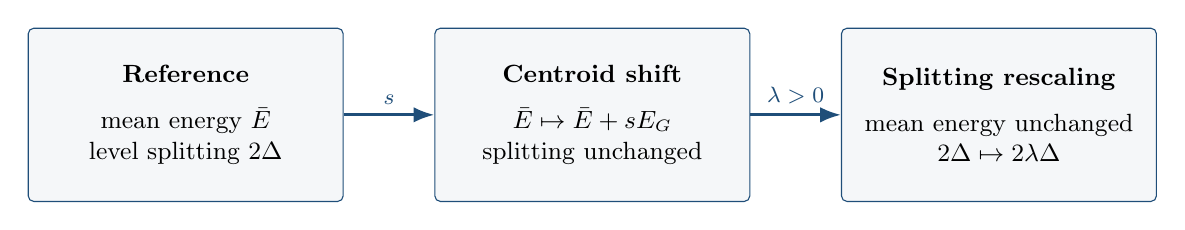
\begin{tikzpicture}[
  >=Latex,
  box/.style={draw=protocolblue,rounded corners=2pt,fill=protocolgray,
              minimum width=4.0cm,minimum height=2.2cm,align=center,
              font=\small},
  arrow/.style={->,line width=1pt,protocolblue},
  note/.style={font=\footnotesize,align=center}
]
  \node[box] (reference) {
    \textbf{Reference}\\[2mm]
    mean energy $\bar E$\\
    level splitting $2\Delta$
  };
  \node[box,right=1.15cm of reference] (shift) {
    \textbf{Centroid shift}\\[2mm]
    $\bar E\mapsto\bar E+sE_G$\\
    splitting unchanged
  };
  \node[box,right=1.15cm of shift] (scale) {
    \textbf{Splitting rescaling}\\[2mm]
    mean energy unchanged\\
    $2\Delta\mapsto2\lambda\Delta$
  };
  \draw[arrow] (reference) -- (shift) node[midway,above,note] {$s$};
  \draw[arrow] (shift) -- (scale) node[midway,above,note] {$\lambda>0$};
\end{tikzpicture}
\caption{Action of the two candidate parameters. A subsequent basis rotation changes
the matrix used for the operator comparison but leaves these energy levels unchanged.
The diagram is schematic and contains no calculated data.}
\label{fig:candidate}
\end{figure}

\subsection{Continuous global alignment family}

The operator comparison allows one global real rotation
\begin{equation}
 R(\phi)=
 \begin{pmatrix}
 \cos\phi&-\sin\phi\\
 \sin\phi& \cos\phi
 \end{pmatrix},
 \qquad
 C_{s,\lambda,\phi}(q)
 =R(\phi)^\dagger C_{s,\lambda}(q)R(\phi).
 \label{eq:global-alignment}
\end{equation}
The same angle is used at every momentum. Momentum-dependent and unrestricted complex
unitary transformations are outside the claim. Since conjugation by
$R(\phi+\pi)=-R(\phi)$ is unchanged, the continuous fundamental interval is
\begin{equation}
 -\frac\pi2\le\phi<\frac\pi2.
 \label{eq:continuous-angle-domain}
\end{equation}
The optimum over this interval is calculated analytically from the second-harmonic
correlation derived below. No finite angle inventory defines the result.

\section{Exact quadratic theory}

\subsection{Loss definitions}

Let $q_i$ be a construction coordinate and $w_i>0$ its raw objective weight. Define
\[
 \alpha_i=\frac{w_i}{\sum_jw_j}.
\]
The canonical input stores the raw weights. A coordinate can be omitted only through a
prospective exclusion rule; a zero weight is not an admissible substitute for exclusion.

For retained rank two, the spectral loss and restricted-alignment matrix loss
(the operator channel) are
\begin{align}
 L_{\mathrm{spec}}^2(s,\lambda)
 &=\sum_i\frac{\alpha_i}{2}
   \sum_{n=1}^{2}
   \left|
   \frac{c_n(q_i;s,\lambda)-h_n(q_i)}{E_G}
   \right|^2,
 \label{eq:spectral-loss}\\
 L_{\mathrm{op},\phi}^2(s,\lambda)
 &=\sum_i\frac{\alpha_i}{2}
   \left\lVert
   \frac{C_{s,\lambda,\phi}(q_i)-A_a(q_i)}{E_G}
   \right\rVert_F^2.
 \label{eq:operator-loss}
\end{align}
To connect the matrix loss to the Bloch states, define the retained-space residual
operator
$\widehat{\Delta H}_{s,\lambda,\phi,a}(k_i)
 =\widehat C_{s,\lambda,\phi}(k_i)-\widehat A_a(k_i)$. In the transported Bloch frame,
\begin{equation}
 [C_{s,\lambda,\phi}(q_i)-A_a(q_i)]_{mn}
 =\langle f_{mq_i}|\widehat{\Delta H}_{s,\lambda,\phi,a}(k_i)
  |f_{nq_i}\rangle.
 \label{eq:operator-residual-bloch-matrix-element}
\end{equation}
Hence the operator channel is the Brillouin-zone weighted root-mean-square of all
retained Bloch-Hamiltonian matrix-element errors, not merely an eigenvalue error. Here
and throughout,
\begin{equation}
 \norm{M}_F^2=\operatorname{tr}(M^\dagger M)=\sum_{m,n}|M_{mn}|^2
 \label{eq:frobenius-definition}
\end{equation}
is the squared Frobenius norm: the sum of the squared magnitudes of every matrix entry.
The factor $1/2$ gives a per-retained-state normalization, and division by $E_G^2$
makes both losses dimensionless.

Define the positive splitting scale
\begin{equation}
 \kappa=
 \sum_i\frac{\alpha_i}{2E_G^2}\norm{D(q_i)}_F^2.
 \label{eq:kappa}
\end{equation}
The nontrivial case has $\kappa>0$, meaning that the retained Hamiltonian is not a scalar
multiple of the identity at every construction coordinate.

For one declared amplitude $a$, suppress the amplitude index on the comparison target.
For an allowed global angle $\phi$, write
\begin{align}
 D_{i,\phi}&=R(\phi)^\dagger D(q_i)R(\phi),\\
 B_i&=U_a(q_i)^\dagger D(q_i)U_a(q_i),\\
 b_\phi&=
 \sum_i\frac{\alpha_i}{2E_G^2}
 \operatorname{Re}\operatorname{tr}(D_{i,\phi}^\dagger B_i),\\
 \mu_\phi&=\frac{b_\phi}{\kappa}.
 \label{eq:operator-correlation}
\end{align}
The scalar $\mu_\phi$ is the normalized correlation between the globally aligned
traceless candidate and the momentum-dependent comparison target.

For a traceless Hermitian $2\times2$ matrix, write
\[
 D_i=x_i\sigma_x+y_i\sigma_y+z_i\sigma_z,
 \qquad
 B_i=X_i\sigma_x+Y_i\sigma_y+Z_i\sigma_z.
\]
Conjugation by a real rotation leaves the $\sigma_y$ component fixed and rotates the
$(\sigma_x,\sigma_z)$ components through angle $2\phi$. Consequently,
\begin{equation}
 b_\phi=b_0+c\cos(2\phi)+d\sin(2\phi),
 \label{eq:correlation-harmonic}
\end{equation}
where
\begin{align}
 b_0&=\sum_i\frac{\alpha_i}{E_G^2}y_iY_i,\\
 c&=\sum_i\frac{\alpha_i}{E_G^2}(x_iX_i+z_iZ_i),\\
 d&=\sum_i\frac{\alpha_i}{E_G^2}(x_iZ_i-z_iX_i).
 \label{eq:harmonic-coefficients}
\end{align}
The exact continuous maximum is
\begin{equation}
 b_{\max}=b_0+\sqrt{c^2+d^2},
 \qquad
 \mu_{\max}=\frac{b_{\max}}{\kappa}.
 \label{eq:continuous-correlation-maximum}
\end{equation}
When $c^2+d^2$ exceeds the declared degeneracy cutoff, a canonical maximizing angle is
\begin{equation}
 \phi_*=\frac12\operatorname{atan2}(d,c)
 \quad\text{reduced to}\quad[-\pi/2,\pi/2).
 \label{eq:continuous-maximizing-angle}
\end{equation}
If the harmonic amplitude is numerically zero, every angle is equally optimal; the
maximum value remains defined but no unique angle is reported.

\subsection{Common-curvature theorem}

\begin{theorem}[Exact loss geometry]
\label{thm:exact-loss-geometry}
Under Eqs.~\eqref{eq:trace-decomposition}--\eqref{eq:operator-correlation}, the losses are
\begin{align}
 L_{\mathrm{spec}}^2(s,\lambda)
 &=s^2+\kappa(\lambda-1)^2,
 \label{eq:exact-spectral-loss}\\
 L_{\mathrm{op},\phi}^2(s,\lambda)
 &=s^2+\kappa(\lambda-\mu_\phi)^2
   +\kappa(1-\mu_\phi^2),
 \label{eq:exact-operator-loss}
\end{align}
and $|\mu_\phi|\le1$. Consequently, the spectral loss and every operator loss have the
same parameter-space curvature
\begin{equation}
 Q=\begin{pmatrix}1&0\\0&\kappa\end{pmatrix}.
 \label{eq:common-curvature}
\end{equation}
The operator component at angle $\phi$ is centered at $(0,\mu_\phi)$ and has irreducible
minimum $m_\phi=\kappa(1-\mu_\phi^2)$. Because the candidate requires $\lambda>0$,
minimizing over the continuous global alignment is equivalent to maximizing $b_\phi$.
The continuously aligned loss is therefore the single quadratic
\begin{equation}
 L_{\mathrm{op},*}^2(s,\lambda)
 =s^2+\kappa(\lambda-\mu_{\max})^2
  +\kappa(1-\mu_{\max}^2).
 \label{eq:continuously-optimized-operator-loss}
\end{equation}
\end{theorem}

\begin{proof}
Let $d_{ia}=h_a(q_i)-\bar E(q_i)$. Since $D(q_i)$ is traceless,
$d_{i1}+d_{i2}=0$. Equation~\eqref{eq:candidate-eigenvalues} gives the normalized
spectral residual
\[
 s+(\lambda-1)d_{ia}/E_G.
\]
When its square is summed over the two retained states, the term linear in $s(\lambda-1)$
vanishes because the two $d_{ia}$ sum to zero. The remaining splitting term is
\[
 \sum_i\frac{\alpha_i}{2E_G^2}\sum_a d_{ia}^2
 =\sum_i\frac{\alpha_i}{2E_G^2}\norm{D(q_i)}_F^2
 =\kappa,
\]
which proves Eq.~\eqref{eq:exact-spectral-loss}.

For the operator channel, Eqs.~\eqref{eq:attacked-matrix} and
\eqref{eq:global-alignment} give the normalized matrix residual
\[
 sI_2+\frac{\lambda D_{i,\phi}-B_i}{E_G}.
\]
The cross term containing $s$ vanishes because both $D_{i,\phi}$ and $B_i$ are
traceless. Unitary invariance of the Frobenius norm gives
$\norm{D_{i,\phi}}_F=\norm{B_i}_F=\norm{D(q_i)}_F$. Expansion therefore yields
\[
 L_{\mathrm{op},\phi}^2
 =s^2+\kappa\lambda^2-2b_\phi\lambda+\kappa.
\]
Completing the square and using $\mu_\phi=b_\phi/\kappa$ proves
Eq.~\eqref{eq:exact-operator-loss}. Finally, Cauchy--Schwarz in the weighted Frobenius
inner product gives $|b_\phi|\le\kappa$, hence $|\mu_\phi|\le1$.
\end{proof}

The theorem identifies the theoretical content of the experiment. Momentum sampling is
needed only to evaluate $\kappa$ and the three harmonic coefficients accurately; it does
not create a collection of independent parent models. The incompatibility mechanism is
$\kappa(1-\mu_{\max}^2)$: it measures the part of the momentum-dependent traceless target
that cannot be represented by one continuously optimized global rotation and one
positive uniform splitting scale.

\section{Exact admissible-set geometry}

Let $\tau_s$ and $\tau_o$ be the spectral and operator error limits. Their values must be
fixed from a stated scientific error budget or identified as synthetic benchmark
controls. Define
\begin{align}
 \mathcal A_s
 &=\{p\in X:L_{\mathrm{spec}}(p)\le\tau_s\},\\
 \mathcal A_o
 &=\{p\in X:L_{\mathrm{op},*}(p)\le\tau_o\}.
 \label{eq:admissible-sets}
\end{align}
The operator ellipse radius in the scaled coordinates is
\begin{equation}
 r_*=
 \sqrt{\tau_o^2-\kappa(1-\mu_{\max}^2)}.
 \label{eq:operator-radius}
\end{equation}
The operator admissible set is empty when the radicand is negative.

Each point $p=(s,\lambda)^T$ in these sets denotes one concrete Bloch-Hamiltonian model:
$sE_G$ is a uniform centroid-energy shift and $\lambda$ is a positive rescaling of the
retained band splitting. Thus $\mathcal A_s$ contains candidates whose band energies
meet the spectral error budget, while $\mathcal A_o$ contains candidates whose retained
Bloch-Hamiltonian matrix elements in the declared frame meet the operator error budget
after one global rotation. A \emph{joint witness} is the same physical candidate
$(s,\lambda)$ belonging to both sets. A separation certificate proves only that no member
of this declared two-parameter candidate family, under the declared global alignment and
error limits, satisfies both requirements. It is not a claim that the complete
Hamiltonians are physically inequivalent, that no larger model class can work, or that a
material phase or topology has been certified. The ellipses live in model-parameter
space, not in the Brillouin zone.

\begin{corollary}[Compatibility and exact full-ellipse distance]
\label{cor:compatibility-distance}
Assume $r_*$ is real and that the spectral and continuously optimized operator ellipses
are contained in the parameter rectangle $X$. They intersect if and only if
\begin{equation}
 \sqrt{\kappa}\,|1-\mu_{\max}|
 \le \tau_s+r_*.
 \label{eq:exact-intersection}
\end{equation}
Their Euclidean distance in $(s,\lambda)$ coordinates is
\begin{equation}
 \delta_*=
 \max\left\{0,
 |1-\mu_{\max}|-\frac{\tau_s+r_*}{\sqrt{\kappa}}
 \right\}.
 \label{eq:exact-distance}
\end{equation}
\end{corollary}

\begin{proof}
Use the scaled coordinates $x=s$ and $y=\sqrt{\kappa}\lambda$. By
Theorem~\ref{thm:exact-loss-geometry}, the spectral ellipse becomes a disk of radius
$\tau_s$ centered at $(0,\sqrt{\kappa})$. The continuously optimized operator ellipse
becomes a disk of radius $r_*$ centered at
$(0,\sqrt{\kappa}\mu_{\max})$. Two disks intersect exactly when the distance between
their centers does not exceed the sum of their radii, which is
Eq.~\eqref{eq:exact-intersection}. Their centers differ only along the splitting
coordinate, so transforming the positive disk gap back to $(s,\lambda)$ coordinates
gives Eq.~\eqref{eq:exact-distance}.
\end{proof}

Thus the theoretical decision is explicit. A common witness exists exactly when
Eq.~\eqref{eq:exact-intersection} holds. Strict separation holds for the full ellipses
when that inequality fails; a resolution-qualified claim additionally requires
\begin{equation}
 \delta_*>\rho_{\mathrm{sep}}
 \label{eq:resolution-qualified-separation}
\end{equation}
with a numerical uncertainty margin.

The containment premise remains scientifically explicit. The formulas above describe
full ellipses, not ellipses clipped by $X$. The calculation verifies all coordinate
extrema before using the corollary as the declared certificate. If containment fails,
the current evidence policy records \emph{invalid premise} or \emph{unresolved}; it does
not silently replace full-ellipse geometry with an unreviewed box-clipped method.

For numerical verification, a general quadratic is still retained in the form
\begin{align}
 r(p)&=r_0+\mathsf Jp,
 &L^2(p)&=p^TQp+2g^Tp+c,\nonumber\\
 Q&=\operatorname{Re}(\mathsf J^\dagger W\mathsf J),
 &g&=\operatorname{Re}(\mathsf J^\dagger Wr_0),
 &c&=\operatorname{Re}(r_0^\dagger Wr_0).
 \label{eq:quadratic}
\end{align}
Here $r_0$ is the stacked complex residual at $p=0$, $\mathsf J$ is its affine
parameter-response matrix, and $W$ contains the declared momentum, retained-state, and
energy-scale weights. For the spectral channel the stacked entries are Bloch-energy
residuals; for the operator channel they are the Bloch-frame matrix elements in
Eq.~\eqref{eq:operator-residual-bloch-matrix-element}. Thus the generic quadratic is an
algebraic representation of the stated Bloch residuals, not a separate fitted model.
The independently reconstructed coefficients must agree with the analytic structure in
Theorem~\ref{thm:exact-loss-geometry}: vanishing cross curvature, unit shift curvature,
common splitting curvature $\kappa$, spectral center $(0,1)$, continuous operator center
$(0,\mu_{\max})$, and agreement of the retained maximizing angle with
Eq.~\eqref{eq:continuous-maximizing-angle}. These identities provide stronger
verification than merely fitting a quadratic to sampled loss values.

\section{Operator information omitted by the Bloch spectrum}

The conventional calculation in Section~\ref{sec:conventional-bloch} retains the
ordered eigenvalues. Applied to the controlled pair $H(q)$ and $A_a(q)$, it finds exact
agreement because
\[
 A_a(q)=U_a(q)^\dagger H(q)U_a(q)
\]
is a unitary conjugation at every momentum. In the candidate family, the same statement
appears as
\begin{equation}
 L_{\mathrm{spec}}(0,1)=0.
 \label{eq:conventional-band-result}
\end{equation}
Thus a band-only calculation accepts the undeformed candidate independently of how
strongly $U(q)$ varies with momentum.

The restricted-alignment matrix question contains information discarded by that
comparison. After exact continuous maximization of the global angle,
Theorem~\ref{thm:exact-loss-geometry} gives the unconstrained best operator residual
\begin{equation}
 \inf_{s\in\mathbb R,\,\lambda\ge0}L_{\mathrm{op},*}^2(s,\lambda)
 =\kappa\left[1-\max(0,\mu_{\max})^2\right].
 \label{eq:operator-blind-spot}
\end{equation}
A strictly positive lower splitting bound can only increase this infimum.
When the momentum-dependent comparison field is exactly representable by one global
rotation, $\mu_{\max}=1$ and the residual vanishes at $(s,\lambda)=(0,1)$. Otherwise,
$1-\mu_{\max}^2$ quantifies the part that a conventional band comparison cannot see and
a single global alignment cannot reproduce.

The same distinction appears in real space. If
\[
 H(q)=\sum_R e^{2\pi iqR}T_R,
 \qquad
 U(q)=\sum_m e^{2\pi iqm}U_m,
\]
then the hopping blocks of $A(q)=U(q)^\dagger H(q)U(q)$ are
\begin{equation}
 \widetilde T_Q=
 \sum_{m,n}U_m^\dagger T_{Q+m-n}U_n.
 \label{eq:gauge-hopping-convolution}
\end{equation}
A momentum-independent basis change has only one nonzero Fourier coefficient and
conjugates each hopping block without changing its range. A momentum-dependent change
mixes displacement indices through Eq.~\eqref{eq:gauge-hopping-convolution}; it can
redistribute weight to longer-range blocks while leaving every band energy unchanged.

The comparison is therefore not between two ways of computing the same band structure.
The conventional calculation answers whether the energies agree. The present theory
asks the stronger question of whether the same restricted candidate also reproduces the
Hamiltonian in a declared frame and the associated hopping representation. The scalar
$\mu_{\max}$ is the exact bridge between those questions for the rank-two family.

\subsection{An exact band-only false positive}

The theory permits an explicit construction in which the conventional band criterion
passes exactly while joint spectral and operator adequacy fails by a positive margin.
This is an analytic counterexample, not a calculated outcome for the four-state parent.

\begin{proposition}[Exact spectral pass with certified operator incompatibility]
\label{prop:constructed-fail}
Consider two equally weighted momentum observations with
\[
 H_1=H_2=\bar E I_2+E_G\sigma_z,
 \qquad
 \sigma_z=\begin{pmatrix}1&0\\0&-1\end{pmatrix},
\]
and comparison rotations
\[
 U_1=R(0),
 \qquad
 U_2=R(\pi/4).
\]
Allow every global real rotation $R(\phi)$ and choose
\[
 X=[-0.20,0.20]\times[0.50,1.10],
 \qquad
 \tau_s=0.05,
 \qquad
 \tau_o=0.72.
\]
Then the conventional spectral loss vanishes at $(s,\lambda)=(0,1)$, but no point in
$X$ satisfies both error limits. The Euclidean separation of the closest full
admissible ellipses is
\begin{equation}
 \delta_*
 =1-\frac{1}{\sqrt2}-0.05
  -\sqrt{0.72^2-\frac12}
 \approx0.1072466192.
 \label{eq:constructed-fail-distance}
\end{equation}
Consequently, any declared separation resolution
$\rho_{\mathrm{sep}}<\delta_*$ is certified.
\end{proposition}

\begin{proof}
For this construction, $\kappa=1$. Conjugation of $\sigma_z$ by a real rotation changes
its orientation through twice the rotation angle. Equation~\eqref{eq:operator-correlation}
therefore gives
\[
 \mu_\phi
 =\frac12\left[\cos(2\phi)+\cos\left(\frac\pi2-2\phi\right)\right]
 =\frac{1}{\sqrt2}\cos\left(2\phi-\frac\pi4\right).
\]
Hence the largest attainable positive correlation is
$\mu_{\max}=1/\sqrt2$, reached at $\phi=\pi/8$. The spectral admissible ellipse is
\[
 s^2+(\lambda-1)^2\le0.05^2.
\]
At the best global angle, the operator ellipse is
\[
 s^2+\left(\lambda-\frac1{\sqrt2}\right)^2
 \le 0.72^2-\frac12.
\]
Both ellipses lie inside $X$. Their centers differ only along the splitting coordinate,
so Corollary~\ref{cor:compatibility-distance} gives
Eq.~\eqref{eq:constructed-fail-distance}.

Angles with smaller positive $\mu_\phi$ cannot reduce the separation: wherever their
operator component is nonempty, decreasing $\mu_\phi$ moves its center farther from
$\lambda=1$ and does not compensate for that shift through its radius. Components with
negative $\mu_\phi$ are either empty at the stated threshold or lie entirely below
$\lambda=0.50$. Thus no allowed global angle produces a joint witness in $X$.
\end{proof}

This construction states precisely what ``the bands pass but the reduced Hamiltonian
fails'' means. The failure is not an optimizer failure: it follows from the exact loss
geometry and a positive certified distance between admissible sets.

\subsection{A smooth continuum of band-equivalent Hamiltonians}

For comparison across the complete reciprocal period, use the smooth periodic family
already defined in Eq.~\eqref{eq:attacked-matrix}:
\begin{equation}
 \mathcal U_{\mathrm{smooth}}
 =\left\{U_a(q)=R\!\left(a\sin 2\pi q\right):
 0\le a\le\frac\pi4\right\}.
 \label{eq:attack-continuum}
\end{equation}
The parameter $a$ is the maximum basis-rotation amplitude. At $a=0$, the comparison and
reference matrices coincide. Increasing $a$ introduces progressively stronger
momentum-to-momentum basis variation while preserving every Bloch eigenvalue exactly.
Unlike a piecewise rotation, Eq.~\eqref{eq:attack-continuum} is smooth and periodic, so
its induced hopping tail reflects a controlled Fourier hierarchy rather than a jump
discontinuity.

For the flat traceless rank-two parent in Eq.~\eqref{eq:flat-traceless-parent}, the
Jacobi--Anger expansion gives the reciprocal-period average
\begin{equation}
 \mu_{\max}(a)=J_0(2a),
 \label{eq:continuum-correlation}
\end{equation}
where $J_0$ is the Bessel function of the first kind~\cite[Sec.~10.12]{dlmf1012}.

\begin{corollary}[Smooth monotone threshold continuum]
\label{cor:threshold-continuum}
For the family in Eq.~\eqref{eq:attack-continuum}, before finite parameter bounds are
applied, the infimum operator threshold is
\begin{equation}
 \tau_{o,\min}(a)
 =\sqrt{\kappa\left[1-J_0(2a)^2\right]}.
 \label{eq:minimum-operator-threshold}
\end{equation}
For a fixed spectral threshold $\tau_s$, the smallest operator threshold permitting a
joint witness is
\begin{equation}
 \tau_{o,\mathrm{joint}}(a;\tau_s)
 =\left[
 \kappa\left[1-J_0(2a)^2\right]
 +\max\!\left\{0,
   \sqrt{\kappa}\left[1-J_0(2a)\right]-\tau_s
  \right\}^{2}
 \right]^{1/2}.
 \label{eq:joint-threshold-continuum}
\end{equation}
For exact spectral acceptance this reduces to
\begin{equation}
 \tau_{o,\mathrm{joint}}(a;0)
 =\sqrt{2\kappa\left[1-J_0(2a)\right]}.
 \label{eq:exact-spectrum-threshold-continuum}
\end{equation}
All three quantities are nondecreasing on $0\le a\le\pi/4$.
\end{corollary}

\begin{proof}
For $D=E_G\sigma_z$, conjugation through Eq.~\eqref{eq:attack-continuum} gives
\[
 U_a(q)^\dagger D U_a(q)
 =E_G\left[
  \cos\!\left(2a\sin2\pi q\right)\sigma_z
  -\sin\!\left(2a\sin2\pi q\right)\sigma_x
 \right].
\]
The sine term has zero reciprocal-period average, while the cosine average is
$J_0(2a)$. A global rotation aligned with $\sigma_z$ therefore maximizes the operator
correlation and proves Eq.~\eqref{eq:continuum-correlation}. Substitution into
Theorem~\ref{thm:exact-loss-geometry} gives
Eq.~\eqref{eq:minimum-operator-threshold}. Solving the exact disk-intersection condition
in Eq.~\eqref{eq:exact-intersection} gives
Eqs.~\eqref{eq:joint-threshold-continuum} and
\eqref{eq:exact-spectrum-threshold-continuum}. On the stated interval, $2a$ remains
before the first positive zero of $J_0$, and $J_0(2a)$ decreases monotonically; the
thresholds therefore increase monotonically.
\end{proof}

\begin{figure}[htbp]
\centering
\begin{tikzpicture}
\begin{axis}[
  width=0.78\textwidth,
  height=0.43\textwidth,
  xmin=0,xmax=0.7853981633974483,
  ymin=0,ymax=1.05,
  xlabel={maximum basis-rotation amplitude $a$},
  ylabel={threshold divided by $\sqrt{\kappa}$},
  xtick={0,0.2617993877991494,0.5235987755982988,0.7853981633974483},
  xticklabels={$0$,$\pi/12$,$\pi/6$,$\pi/4$},
  legend style={at={(0.03,0.97)},anchor=north west,draw=none,fill=white},
  axis lines=left,
  grid=major,
  grid style={black!10}
]
\addplot[protocolblue,very thick]
 table[x=a,y=operator_threshold_over_sqrt_kappa,col sep=comma]
 {smooth-threshold-continuum.csv};
\addlegendentry{$\tau_{o,\min}/\sqrt\kappa$}
\addplot[red!70!black,very thick,dashed]
 table[x=a,y=joint_threshold_over_sqrt_kappa,col sep=comma]
 {smooth-threshold-continuum.csv};
\addlegendentry{$\tau_{o,\mathrm{joint}}(a;0)/\sqrt\kappa$}
\end{axis}
\end{tikzpicture}
\caption{Analytic acceptance thresholds for the smooth continuum in
Eq.~\eqref{eq:attack-continuum}. Every amplitude has exactly the same Bloch bands. The
solid curve is the smallest threshold admitting an operator fit before finite parameter
bounds are applied. The dashed curve additionally requires exact spectral agreement.
The plotted points are evaluations of the displayed Bessel formulas, not empirical
data.}
\label{fig:threshold-continuum}
\end{figure}

This family supports a direct side-by-side calculation across $a$: the conventional
branch reports zero band change, while the representation-aware branch reports the
operator threshold and the induced Fourier hopping tail.

\section{Exact relation to representation-induced hopping range}

The threshold has a direct real-space meaning. Consider the spectrally flat traceless
parent
\begin{equation}
 H(q)=\bar E I_2+D,
 \qquad D=D^T\in\mathbb R^{2\times2},
 \qquad \operatorname{tr}D=0,
 \qquad D\ne0,
 \label{eq:flat-traceless-parent}
\end{equation}
where $\bar E$ and $D$ are independent of momentum. Its only hopping block is onsite.
After a momentum-dependent real rotation, the traceless comparison field is
\begin{equation}
 B(q)=U(q)^\dagger D U(q).
 \label{eq:rotated-traceless-field}
\end{equation}
Define its Fourier blocks by
\begin{equation}
 B_R=\int_{-1/2}^{1/2}e^{-2\pi iqR}B(q)\,dq,
 \qquad
 B(q)=\sum_{R\in\mathbb Z}e^{2\pi iqR}B_R.
 \label{eq:continuous-traceless-fourier}
\end{equation}
The nonzero-$R$ blocks are hopping terms created entirely by the momentum dependence of
the basis transformation.

\begin{theorem}[Operator residual equals induced nonlocal hopping weight]
\label{thm:residual-locality-identity}
Let $B(q)$ be given by Eq.~\eqref{eq:rotated-traceless-field}, with $U(q)$ restricted to
the same real two-dimensional rotation family as the allowed global alignment. Set
\begin{equation}
 \kappa=\frac{\norm{D}_F^2}{2E_G^2},
 \qquad
 \mu_{\max}=\frac{\norm{B_0}_F}{\norm{D}_F}.
 \label{eq:locality-kappa-mu}
\end{equation}
Then
\begin{align}
 \inf_{s\in\mathbb R,\,\lambda\ge0,\,\phi}
 L_{\mathrm{op},\phi}^2(s,\lambda)
 &=\kappa(1-\mu_{\max}^2)
 \label{eq:residual-locality-left}\\
 &=\frac{1}{2E_G^2}
   \sum_{R\ne0}\norm{B_R}_F^2.
 \label{eq:residual-locality-right}
\end{align}
Thus the squared irreducible operator residual is exactly the normalized Fourier weight
outside the onsite block. For a finite uniform mesh, the same identity holds with the
integral and Fourier series replaced by the corresponding discrete transform.
\end{theorem}

\begin{proof}
Every matrix $U(q)^\dagger D U(q)$ is traceless, has Frobenius norm $\norm D_F$, and lies
in the two-dimensional real rotation orbit of $D$. Its average $B_0$ lies in the disk
spanned by that orbit. Hence there are a global angle $\phi_0$ and a scale
$\lambda_0\ge0$ such that
\[
 B_0=\lambda_0R(\phi_0)^\dagger D R(\phi_0),
 \qquad
 \lambda_0=\frac{\norm{B_0}_F}{\norm{D}_F}=\mu_{\max}.
\]
The best constant globally aligned field is therefore the orthogonal projection $B_0$.
The trace shift is minimized by $s=0$, and
\begin{equation}
 \inf_{s,\lambda,\phi}L_{\mathrm{op},\phi}^2
 =\frac{1}{2E_G^2}
  \int_{-1/2}^{1/2}\norm{B(q)-B_0}_F^2\,dq.
 \label{eq:mean-field-residual}
\end{equation}
Parseval's identity applied entrywise to
Eq.~\eqref{eq:continuous-traceless-fourier} turns the right side into the nonzero-mode
sum in Eq.~\eqref{eq:residual-locality-right}. Unitary invariance gives
$\norm{B(q)}_F=\norm{D}_F$ pointwise, so a second application of Parseval gives
\[
 \sum_{R\ne0}\norm{B_R}_F^2
 =\norm D_F^2-\norm{B_0}_F^2
 =\norm D_F^2(1-\mu_{\max}^2).
\]
Division by $2E_G^2$ proves Eq.~\eqref{eq:residual-locality-left}.
\end{proof}

For the smooth continuum in Eq.~\eqref{eq:attack-continuum},
$\mu_{\max}(a)=J_0(2a)$. The theorem therefore gives
\begin{equation}
 \frac{1}{2E_G^2}\sum_{R\ne0}\norm{B_R(a)}_F^2
 =\kappa\left[1-J_0(2a)^2\right]
 =\tau_{o,\min}(a)^2.
 \label{eq:continuum-tail-identity}
\end{equation}
The solid curve in Fig.~\ref{fig:threshold-continuum} is consequently the square root of
the induced non-onsite hopping weight. If exact spectral agreement additionally fixes
$\lambda=1$, the joint threshold contains a second contribution from the mismatch of
the onsite block:
\begin{equation}
 \tau_{o,\mathrm{joint}}(a;0)^2
 =\underbrace{\kappa\left[1-J_0(2a)^2\right]}_{\text{non-onsite hopping weight}}
 +\underbrace{\kappa\left[1-J_0(2a)\right]^2}_{\text{onsite-block mismatch}}.
 \label{eq:joint-threshold-locality-decomposition}
\end{equation}

This identity is the substantive distinction from a band-only diagnostic. The band
energies remain unchanged, but the momentum-dependent representation necessarily moves
a calculable amount of operator weight outside the cell-local block. A global rotation
can change the orbital basis within each cell but cannot remove those nonzero-range
Fourier blocks.

\section{Side-by-side Bloch and representation-aware calculation}

The computational study evaluates the same continuum through two branches. Both branches
start from one solution of the parent Bloch eigenproblem. The parent is not refitted or
rediagonalized as a different physical model at each amplitude.

\subsection{Conventional Bloch branch}

For every amplitude $a$ and momentum $q_i$, construct $A_a(q_i)$ from
Eq.~\eqref{eq:attack-continuum} and independently diagonalize it. Record the ordered-band
defect
\begin{equation}
 \Delta_{\mathrm{band}}(a)
 =\max_{i,n}
 \frac{|\varepsilon_n[A_a(q_i)]-\varepsilon_n[H(q_i)]|}{E_G}.
 \label{eq:band-continuum-defect}
\end{equation}
The analytic value is zero for every $a$; the calculated value measures only numerical
eigensolver and ordering error. The branch also records the two overlaid band curves at
selected amplitudes. No operator matrix element or hopping block enters its acceptance
criterion.

\subsection{Representation-aware branch}

Using the same matrices $A_a(q_i)$, calculate
\begin{enumerate}[label=\arabic*.]
  \item the best global alignment correlation $\mu_{\max}(a)$;
  \item the irreducible operator loss
        $L_{\mathrm{op,min}}(a)$;
  \item the operator threshold required for a joint witness at each declared spectral
        threshold;
  \item the Fourier hopping blocks $\widetilde T_R(a)$; and
  \item the range-resolved tail
        \begin{equation}
        P_{>R_c}(a)=\frac{1}{2E_G^2}
        \sum_{|R|>R_c}\norm{\widetilde T_R(a)}_F^2.
        \label{eq:continuum-hopping-tail}
        \end{equation}
\end{enumerate}
For the flat analytic parent, $R_c=0$ and
\begin{equation}
 L_{\mathrm{op,min}}(a)^2=P_{>0}(a)
 =\kappa\left[1-J_0(2a)^2\right].
 \label{eq:continuum-three-way-identity}
\end{equation}
The calculation retains the defect in this three-way identity as a verification channel.
For the finite-range four-state realization, the parent itself has nonzero-range blocks;
the analysis therefore reports the complete range-resolved distribution and its change
with $a$, without assuming that Eq.~\eqref{eq:continuum-three-way-identity} continues to
hold unchanged.

\subsection{Continuum sampling and comparison figures}

The proposed amplitude interval is $0\le a\le\pi/4$. A nested amplitude study uses
\begin{equation}
 a_j=\frac{j\pi}{4N_a},
 \qquad j=0,\ldots,N_a,
 \qquad N_a\in\{8,16,32,64\}.
 \label{eq:amplitude-mesh}
\end{equation}
Coarse amplitudes reappear on every doubled grid. Convergence is required for
$\mu_{\max}$, the operator thresholds, and every reported hopping-tail channel.
Comparing only shared amplitude nodes is insufficient because those values agree by
construction. A current exploratory midpoint-interpolation analysis finds maximum
defects $3.08\times10^{-5}$ and $1.41\times10^{-5}$ for the two threshold curves at
$N_a=64$, above the draft unit-scale tolerance $1.01\times10^{-8}$. The ladder in
Eq.~\eqref{eq:amplitude-mesh} therefore remains a proposal and must not be frozen. This
finding does not require a uniform 4096-interval grid if the final protocol instead
evaluates the analytic law directly or adopts a reviewed adaptive amplitude rule. The
initial non-flat study independently confirms that the same proposed ladder is
insufficient: at $N_a=64$, its largest correlation and hopping-block midpoint defects
are $3.49\times10^{-5}$ and $1.39\times10^{-5}$, respectively. No flat-parent analytic
comparator is used for those non-flat defects. The deterministic adaptive action caches
direct samples, evaluates interval midpoints, refines only failing intervals, and then
requires disjoint quarter-point validation. It remains `unresolved' when its explicit
level or unique-sample cap is reached. Its production cap and thresholds are not frozen.

The composite comparison in Fig.~\ref{fig:flat-parent-analysis} places conventional
Bloch bands, operator-acceptance thresholds, amplitude resolution, cumulative tails, and
range-resolved hopping weight in one view. The intended contrast is quantitative: the
bands remain unchanged, while the representation-aware panels resolve the increasing
operator mismatch and representation-induced hopping range.

\section{Exploratory flat-parent analysis}
\label{sec:exploratory-analysis}

Figure~\ref{fig:flat-parent-analysis} summarizes the pre-version calculation for the
normalized smooth flat-parent family. It is a development result generated by the
current software implementation; it is not a retained run or an evidence package.

\begin{figure}[p]
  \centering
  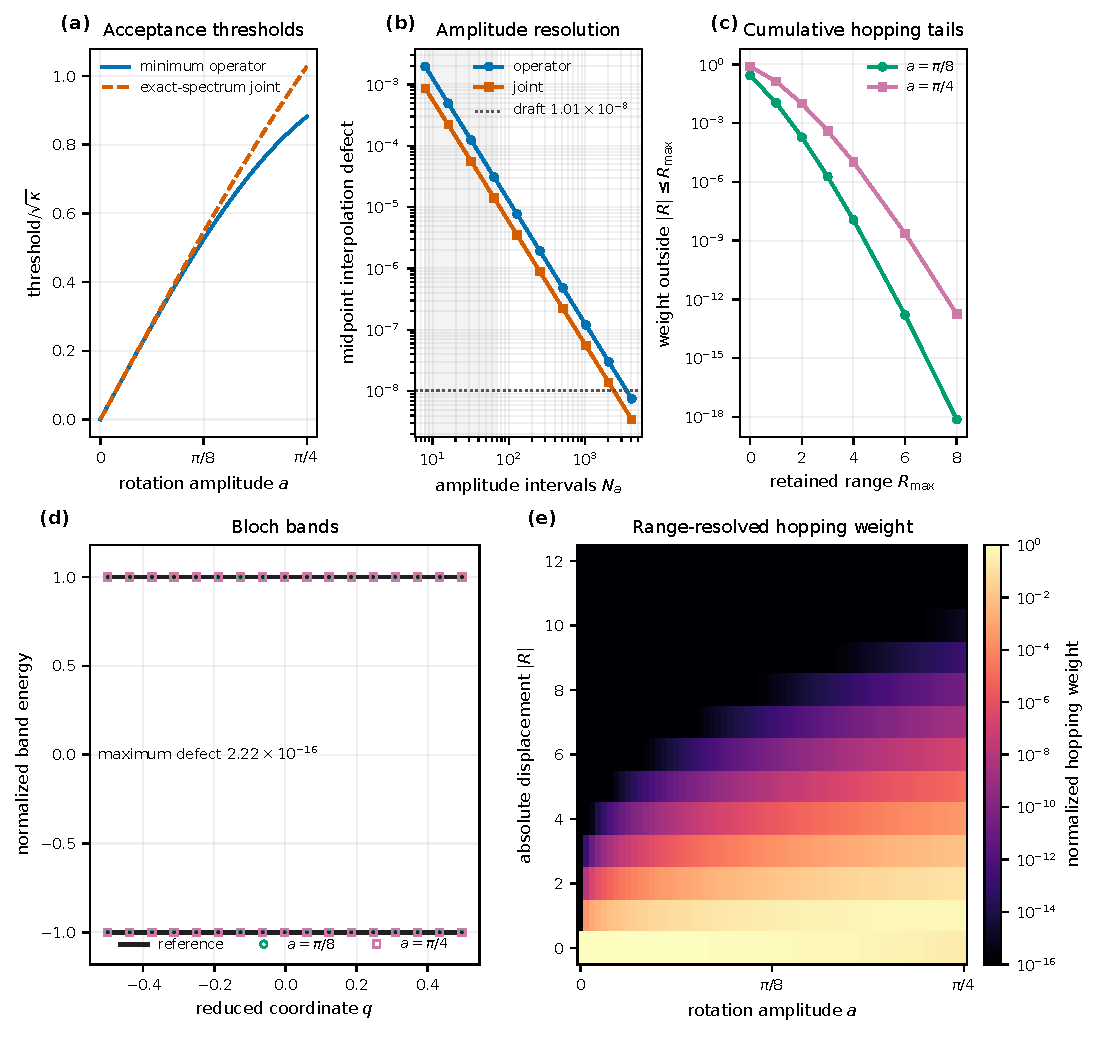
\includegraphics[width=\textwidth]
    {analysis/band-equivalence-versus-hopping-locality.pdf}
  \caption{Band equivalence versus hopping locality in the smooth flat-parent
  continuum. \textbf{(a)} Normalized minimum operator and exact-spectrum joint
  acceptance thresholds as functions of the maximum rotation amplitude $a$.
  \textbf{(b)} Maximum midpoint defect of piecewise-linear interpolation on nested
  uniform amplitude grids; the shaded region marks the proposed $N_a=8$--64 ladder,
  and the dotted line is the draft $1.01\times10^{-8}$ unit-scale target.
  \textbf{(c)} Cumulative normalized hopping weight outside the retained range
  $|R|\le R_{\max}$ for two amplitudes. \textbf{(d)} Reference and transformed Bloch
  bands; the largest computed eigenvalue defect is $2.22\times10^{-16}$.
  \textbf{(e)} Normalized range-resolved hopping weight over amplitude and absolute
  displacement. Thresholds in panel (a) use the analytic $J_0(2a)$ comparator; panels
  (c) and (e) use the $N=512$ finite transform after nested momentum refinement. The
  calculation shown is pre-version development analysis and is not a retained evidence
  run.}
  \label{fig:flat-parent-analysis}
\end{figure}

The reference and transformed models retain the same Bloch eigenvalues across the
Brillouin zone. Their largest calculated band defect is
$2.22\times10^{-16}$ [Fig.~\ref{fig:flat-parent-analysis}(d)], so the conventional band
structure does not distinguish the two representations. The representation-aware
thresholds nevertheless increase continuously with amplitude
[Fig.~\ref{fig:flat-parent-analysis}(a)]. Equations~\eqref{eq:minimum-operator-threshold}
and \eqref{eq:exact-spectrum-threshold-continuum} give normalized minimum-operator and
exact-spectrum joint thresholds of $0.8815978972$ and $1.0276174232$, respectively, at
$a=\pi/4$. Their separation shows that exact band agreement does not remove the
operator-level cost of identifying the representations.

The same mismatch appears in real-space locality. At $a=0$, all normalized hopping
weight outside the onsite block is below $1.3\times10^{-28}$ on the $N=512$ transform.
The total non-onsite weight rises to $0.2747231$ at $a=\pi/8$ and $0.7772149$ at
$a=\pi/4$. The cumulative tails in Fig.~\ref{fig:flat-parent-analysis}(c) decay rapidly
with retained range, but their amplitude dependence is pronounced: the weight outside
$|R|\le4$ is $1.16\times10^{-8}$ at $a=\pi/8$ and $1.03\times10^{-5}$ at $a=\pi/4$.
The range-resolved map in Fig.~\ref{fig:flat-parent-analysis}(e) confirms that the support
broadens continuously even though the bands remain unchanged. This is the calculated
counterpart of the exact flat-parent identity in
Eq.~\eqref{eq:continuum-three-way-identity}.

The numerical study separates momentum and amplitude resolution. For the implemented
flat-parent channels, refinement from $N=32$ through $N=512$ changes every monitored
momentum-dependent quantity only at approximately binary64 roundoff. By contrast, the
proposed uniform amplitude ladder
through $N_a=64$ is insufficient to reconstruct a continuous threshold curve at the
draft $1.01\times10^{-8}$ level [Fig.~\ref{fig:flat-parent-analysis}(b)]. Its maximum
midpoint interpolation defects are $3.08\times10^{-5}$ and $1.41\times10^{-5}$ for the
operator and joint thresholds. The first tested uniform grid to pass the draft target
has $N_a=4096$. This does not imply that every calculation requires 4096 amplitudes: the
analytic flat-parent laws can be evaluated directly, while a non-analytic realization
should use a reviewed adaptive rule rather than infer between-node convergence from
shared nested nodes alone.

This benchmark establishes the analytic mechanism and tests the implemented flat-parent
correlation, threshold, band-defect, and Fourier-locality channels, but it does not test
the prospective frame, admissible-set, witness, or separation-certificate workflow and
does not establish material realism. The parent is deliberately flat, and the reported
hopping blocks are finite-mesh Fourier coefficients. A qualified non-flat realization
and a frozen retained run remain necessary before these numerical values can serve as
final publication evidence.

\section{Exploratory non-flat four-state analysis}
\label{sec:nonflat-exploratory}

The initial typed implementation constructs the parent in
Eq.~\eqref{eq:parent-bloch}, selects the lower two-state spectral subspace, closes the
parallel-transport frame, and applies Eq.~\eqref{eq:attacked-matrix}. Figure~\ref{fig:nonflat-analysis}
reports the resulting pre-version diagnostics. They are neither retained evidence nor a
converged numerical result.

\begin{figure}[p]
  \centering
  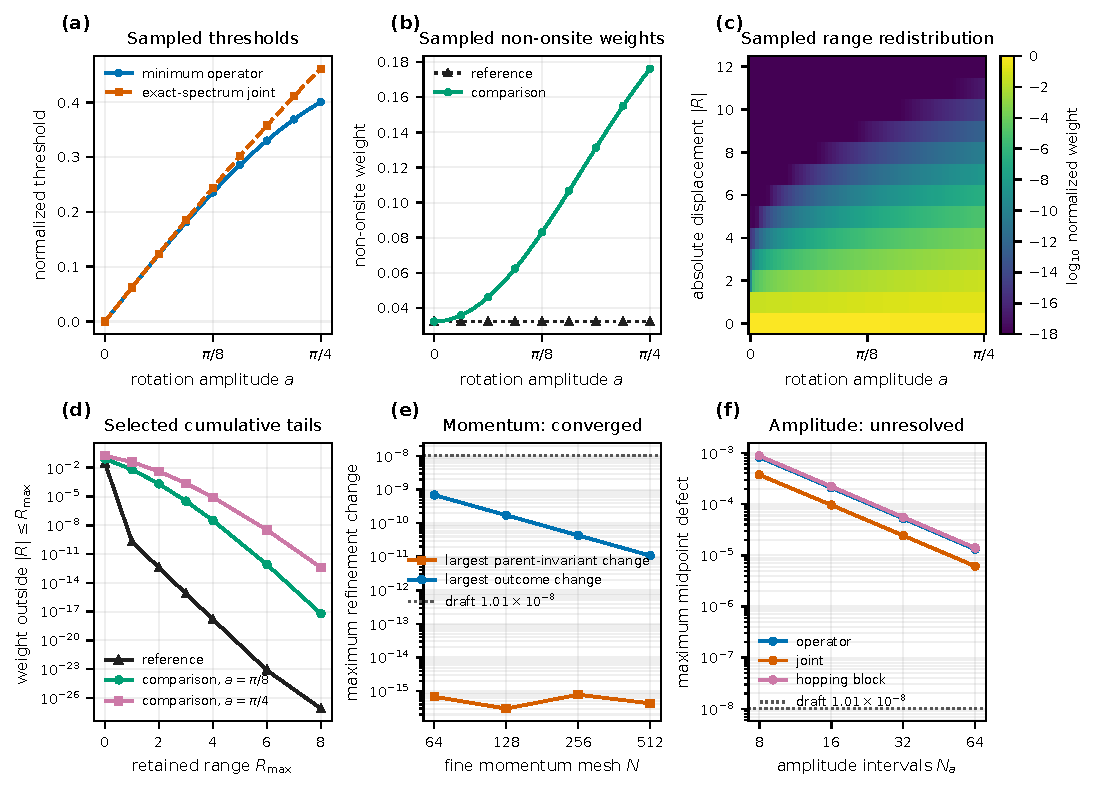
\includegraphics[width=\textwidth]
    {analysis/nonflat-four-state-exploratory.pdf}
  \caption{Exploratory smooth non-flat four-state realization. \textbf{(a)}
  Restricted-alignment minimum-operator and exact-spectrum joint thresholds over a
  65-node sampling of the smooth amplitude family. Markers show every eighth direct
  sample and connecting lines are guides to the eye. \textbf{(b)} Reference and
  comparison non-onsite weights over the same samples.
  \textbf{(c)} Range-resolved comparison hopping redistribution over amplitude and
  absolute displacement. \textbf{(d)} Selected cumulative finite-mesh hopping tails.
  \textbf{(e)} Adjacent momentum-refinement changes: both parent-invariant and selected
  outcome channels lie below the draft target. \textbf{(f)}
  Midpoint amplitude-interpolation defects, all above the draft target on the tested
  $N_a\le64$ ladder. No $J_0(2a)$ comparator or flat-parent residual--tail identity is
  used. Momentum refinement is `converged', amplitude interpolation is `unresolved',
  and the calculation is not a retained evidence run.}
  \label{fig:nonflat-analysis}
\end{figure}

At $N=512$, the minimum sampled external gap is $1.0566461$, the minimum neighboring-frame
transport singular value is $0.9999997323$, and the largest independently reconstructed
result defect is $3.09\times10^{-15}$. The largest computed band defect over 65
amplitudes is $1.45\times10^{-15}$. At $a=\pi/4$, the discrete maximum correlation is
$0.5079908088$, the minimum operator threshold is $0.4004394264$, and the exact-spectrum
joint threshold is $0.4611609032$ [Fig.~\ref{fig:nonflat-analysis}(a)]. The comparison
non-onsite hopping weight increases from the reference value $0.0323839143$ to
$0.1761532501$. Its weight outside $|R|\le4$ is $8.43\times10^{-6}$, whereas the
reference value is $1.52\times10^{-18}$ [Fig.~\ref{fig:nonflat-analysis}(d)]. The full
amplitude-dependent redistribution is shown in
Figs.~\ref{fig:nonflat-analysis}(b)--(c). These are
finite-mesh observations, not the flat-parent identity in
Eq.~\eqref{eq:continuum-three-way-identity}.

The momentum disposition is `converged'. Between $N=256$ and $N=512$, the largest
selected outcome-channel change is $1.08\times10^{-11}$ and the largest
parent-invariant change is $1.67\times10^{-16}$
[Fig.~\ref{fig:nonflat-analysis}(e)]. Neighboring-frame overlap remains a qualification
lower bound rather than a convergence observable; shared parent eigenvalues and retained
spectral projectors provide the invariant cross-mesh checks. At $N_a=64$, the
largest correlation midpoint defect is $3.49\times10^{-5}$ and the largest
hopping-block-power midpoint defect is $1.39\times10^{-5}$
[Fig.~\ref{fig:nonflat-analysis}(f)]. The failing amplitude control is not overridden by
momentum convergence, roundoff-level band agreement, or apparently stable selected
thresholds.

\subsection{Bounded parent-family robustness study}

To distinguish the representation orbit from dependence on one selected parent, define
\begin{equation}
 K_\rho(q)=T_0+\rho\left(e^{2\pi iq}T_{+1}+e^{-2\pi iq}T_{-1}\right),
 \qquad 0\leq\rho\leq1.
 \label{eq:parent-homotopy}
\end{equation}
Thus $\rho=0$ is the onsite four-state parent and $\rho=1$ is the full parent in
Eq.~\eqref{eq:parent-bloch}. The onsite matrices, retained rank, frame protocol, and
rotation family are unchanged. Every sampled $\rho$ must independently clear the gap,
transport-rank, reconstruction, and momentum-refinement controls.

\begin{figure}[p]
  \centering
  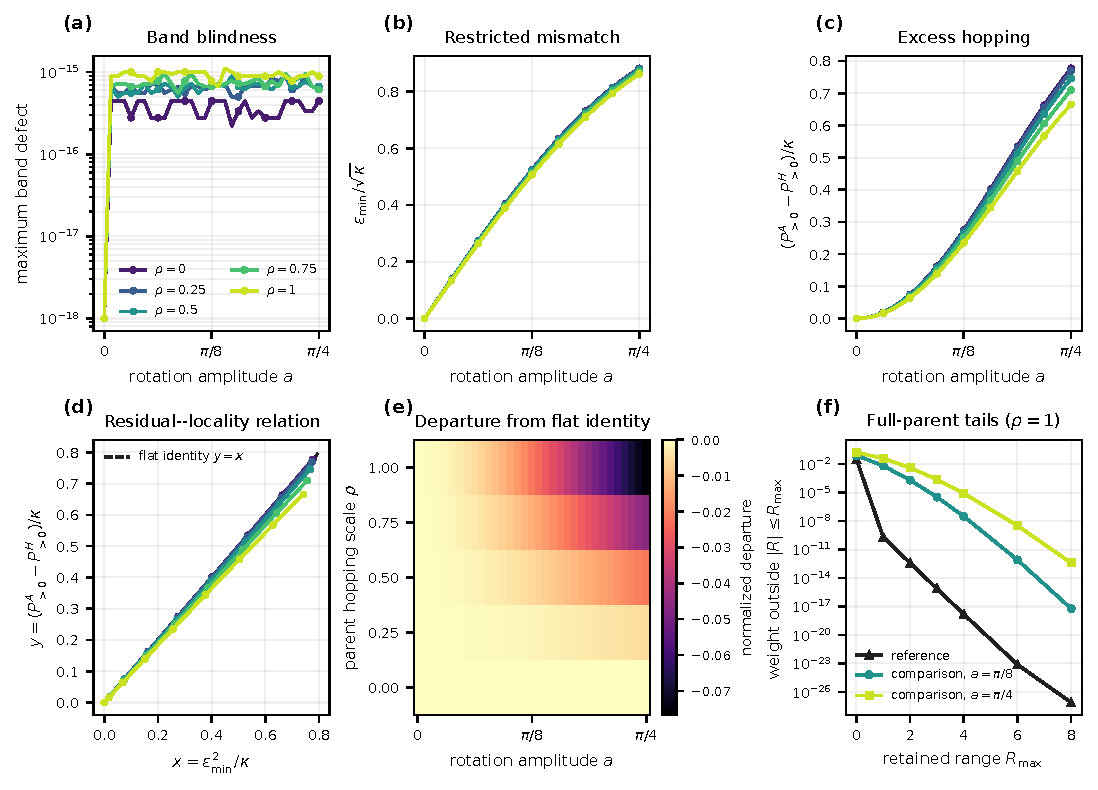
\includegraphics[width=\textwidth]
    {analysis/band-equivalence-locality-scientific-story.pdf}
  \caption{Band equivalence and locality across the sampled parent family.
  \textbf{(a)} Maximum ordered-eigenvalue defect; exact zeros are displayed at
  $10^{-18}$ on the logarithmic axis. \textbf{(b)} Minimum restricted-alignment
  threshold normalized by $\sqrt{\kappa}$; the dashed curve is the analytic flat-parent
  comparator. \textbf{(c)} Comparison-minus-reference non-onsite weight normalized by
  $\kappa$, with the flat analytic identity shown dashed. \textbf{(d)} Parametric
  relation between normalized squared operator residual $x$ and normalized excess
  locality weight $y$; the dashed diagonal is the flat identity $y=x$.
  \textbf{(e)} Directly calculated departure $y-x$ over the $5\times33$ sampled
  parameter pairs. \textbf{(f)} Full-parent cumulative tails at selected amplitudes.
  Colors identify the parent hopping scales in panel (a), markers show every fourth
  amplitude sample, and connecting lines are guides to the eye. All five momentum
  studies through $N=256$ are `converged'; the finite $\rho$ and amplitude inventories
  are not continuous-domain certificates. This is a pre-version development
  calculation, not a retained evidence run or material validation.}
  \label{fig:parent-family-analysis}
\end{figure}

\subsection{Implemented metrics and interpretation of the parent-family figure}

The implemented calculation concerns complete finite-mesh retained Hamiltonians, not
range-truncated approximations. For each sampled parent scale $\rho$, the four-state
parent is diagonalized, the lower two-dimensional spectral subspace is transported into
a periodic orthonormal frame, and the resulting $2\times2$ retained field $H_\rho(q_i)$
is formed. The comparison field is
\begin{equation}
 A_{\rho,a}(q_i)=U_a(q_i)^\dagger H_\rho(q_i)U_a(q_i),
 \qquad U_a(q)=R(a\sin 2\pi q).
 \label{eq:implemented-parent-family-comparison}
\end{equation}
Equation~\eqref{eq:implemented-parent-family-comparison} is a pointwise unitary change of
representation. The complete reference and comparison fields therefore have identical
ordered eigenvalues in exact arithmetic. The reported band defect is
\begin{equation}
 \Delta_{\mathrm{band}}(\rho,a)=
 \max_{i,n}\frac{|\varepsilon_n[A_{\rho,a}(q_i)]
                       -\varepsilon_n[H_\rho(q_i)]|}{E_G}.
 \label{eq:implemented-band-defect}
\end{equation}
It is a numerical confirmation of the constructed similarity relation, not evidence that
two independently derived material Hamiltonians agree. Exact zeros in
Fig.~\ref{fig:parent-family-analysis}(a) are placed at $10^{-18}$ only for logarithmic
display.

Let $H_\rho^\circ(q_i)$ denote the traceless retained field and define
\begin{equation}
 \kappa_\rho=\frac{1}{N}\sum_i
 \frac{\|H_\rho^\circ(q_i)\|_F^2}{2E_G^2}.
 \label{eq:implemented-splitting-scale}
\end{equation}
The continuous harmonic maximization gives the largest normalized correlation
$\mu_{\rho,a,\max}$ attainable by one momentum-independent real rotation. The candidate
also admits one positive splitting multiplier. Its irreducible matrix-loss threshold is
\begin{equation}
 \epsilon_{\min}(\rho,a)
 =\sqrt{\kappa_\rho\left[1-\max(0,\mu_{\rho,a,\max})^2\right]}.
 \label{eq:implemented-minimum-threshold}
\end{equation}
Consequently, panel (b) plots $\epsilon_{\min}/\sqrt{\kappa_\rho}$ and panel (d) uses
\begin{equation}
 x=\frac{\epsilon_{\min}^2}{\kappa_\rho}.
 \label{eq:implemented-normalized-residual}
\end{equation}
This metric answers a restricted representation question: how much of the
momentum-dependent comparison field cannot be reproduced by one global real rotation,
one positive scale, and the common mean-energy field. It is not a distance between
abstract operators under arbitrary momentum-dependent unitary equivalence.

For centered finite-mesh cell displacements, the implementation constructs Fourier
blocks $T_R^{H_\rho}$ and $T_R^{A_{\rho,a}}$. In the Wannier representation generated
by the chosen periodic Bloch frame, their entries have the tight-binding meaning
\begin{equation}
 [T_R^X]_{mn}=\langle 0m|\widehat X|Rn\rangle,
 \qquad
 X_{mn}(q)=\sum_R e^{2\pi iqR}[T_R^X]_{mn},
 \label{eq:implemented-wannier-hopping}
\end{equation}
where $|Rn\rangle$ is the Wannier orbital in cell $R$ associated with retained orbital
$n$. On the finite construction mesh this is a discrete, potentially aliased Wannier
representation rather than a continuous localization certificate. A momentum-dependent
Bloch-frame rotation corresponds to mixing Wannier orbitals across lattice cells. It can
therefore redistribute the real-space matrix elements in
Eq.~\eqref{eq:implemented-wannier-hopping} without changing the complete Bloch spectrum.
The implementation assigns each block the per-retained-state power
\begin{equation}
 p_R^X=\frac{\|T_R^X\|_F^2}{2E_G^2},
 \qquad
 P_{>0}^X=\sum_{R\ne0}p_R^X,
 \qquad X\in\{H_\rho,A_{\rho,a}\}.
 \label{eq:implemented-hopping-power}
\end{equation}
Panel (c) plots the signed excess
\begin{equation}
 y=\frac{P_{>0}^{A_{\rho,a}}-P_{>0}^{H_\rho}}{\kappa_\rho}.
 \label{eq:implemented-normalized-excess}
\end{equation}
Equivalently,
\begin{equation}
 p_R^X=\frac{1}{2E_G^2}\sum_{m,n}
 |\langle 0m|\widehat X|Rn\rangle|^2.
 \label{eq:implemented-hopping-power-matrix-elements}
\end{equation}
Thus $p_R^X$ is an entrywise squared-amplitude diagnostic for hopping between cell
Wannier orbitals, summed over all retained-orbital pairs and normalized per retained
state and by $E_G^2$. It is not a transition probability. Although both terms in the
numerator are nonnegative,
their difference is not a norm and need not be nonnegative for an arbitrary family. It
is positive for the sampled family.
At $\rho=0$, the reference has no non-onsite hopping and the flat-parent theorem gives
$y=x$. For $\rho>0$, the reference already contains non-onsite blocks. Writing
$T_R^{A}=T_R^{H}+\delta T_R$ shows that the excess contains both
$\|\delta T_R\|_F^2$ and the cross term
$2\operatorname{Re}\operatorname{tr}[(T_R^H)^\dagger\delta T_R]$. No theorem therefore
identifies $y$ with the restricted residual $x$ for a dispersive parent. Panels (d) and
(e) report the calculated relation and the diagnostic departure $y-x$ rather than
assuming the flat identity. The systematic negative departure means that the increase in
non-onsite block power accounts for less than the full normalized restricted residual in
this family; it is not a failure of band equivalence.

Finally, panel (f) reports
\begin{equation}
 P_{>R_c}^{X}=\sum_{|R|>R_c}p_R^X
 \label{eq:implemented-cumulative-tail}
\end{equation}
for the full parent $\rho=1$ at selected amplitudes. This is the hopping power that a
symmetric range cutoff would omit. The complete-model calculation underlying panel (f)
does not itself construct a truncated Hamiltonian. Thus panel (f) measures
representation-dependent real-space compactness, not a spectral truncation error. The
separate truncation consequence action below tests the spectral effect explicitly.

The figure matters for reduced solid-state modeling because the gauge of a retained
subspace controls how economically its complete Bloch field can be represented by
real-space hopping blocks. Panels (a)--(e) show that exact band equivalence can coexist
with a large restricted representation residual and a redistribution of hopping power,
and that this conclusion survives the sampled introduction of parent dispersion. They
do not establish physical inequivalence of the complete gauge-related Hamiltonians. The
parent homotopy is synthetic, the five $\rho$ values and 33 amplitudes are finite direct
samples, and the coefficients remain finite-mesh Fourier coefficients rather than a
continuous-domain or material-localization certificate.

All five momentum studies return `converged'. The smallest sampled external gap decreases
from $1.3436583E_G$ at $\rho=0$ to $1.0566461E_G$ at $\rho=1$, while the reference
non-onsite weight rises from numerical noise to $0.0323839$. At $a=\pi/4$, the
scale-normalized minimum threshold changes from $0.8815979$ to $0.8613625$, and the
excess comparison non-onsite weight changes from $0.1431824$ to $0.1437693$
[Fig.~\ref{fig:parent-family-analysis}(b)--(c)]. The normalized flat-identity departure
$y-x$ changes from roundoff at $\rho=0$ to $-0.0767265$ at $\rho=1$
[Fig.~\ref{fig:parent-family-analysis}(d)--(e)]. Thus the restricted mismatch and excess
hopping remain large while the exact flat residual--tail identity deforms systematically
with parent dispersion. The representation-induced mismatch is therefore observed
throughout the sampled homotopy, not only for the endpoint parent.
The five $\rho$ values and 33 amplitudes remain finite samples; they do not establish a
continuous-$\rho$ bound or resolve amplitude interpolation.

\subsection{Exploratory finite-range band consequences}

The consequence action uses $N=256$, the $M=1025$ disjoint evaluation mesh, the same
five parent scales and 33 pointwise amplitudes, and
$R_c\in\{0,1,2,3,4,6,8,12,16,24,32,48,64\}$. These are development samples rather than
a frozen retained inventory. The minimum periodic separation between the construction
and evaluation meshes is $1.48\times10^{-8}$.

\begin{figure}[p]
  \centering
  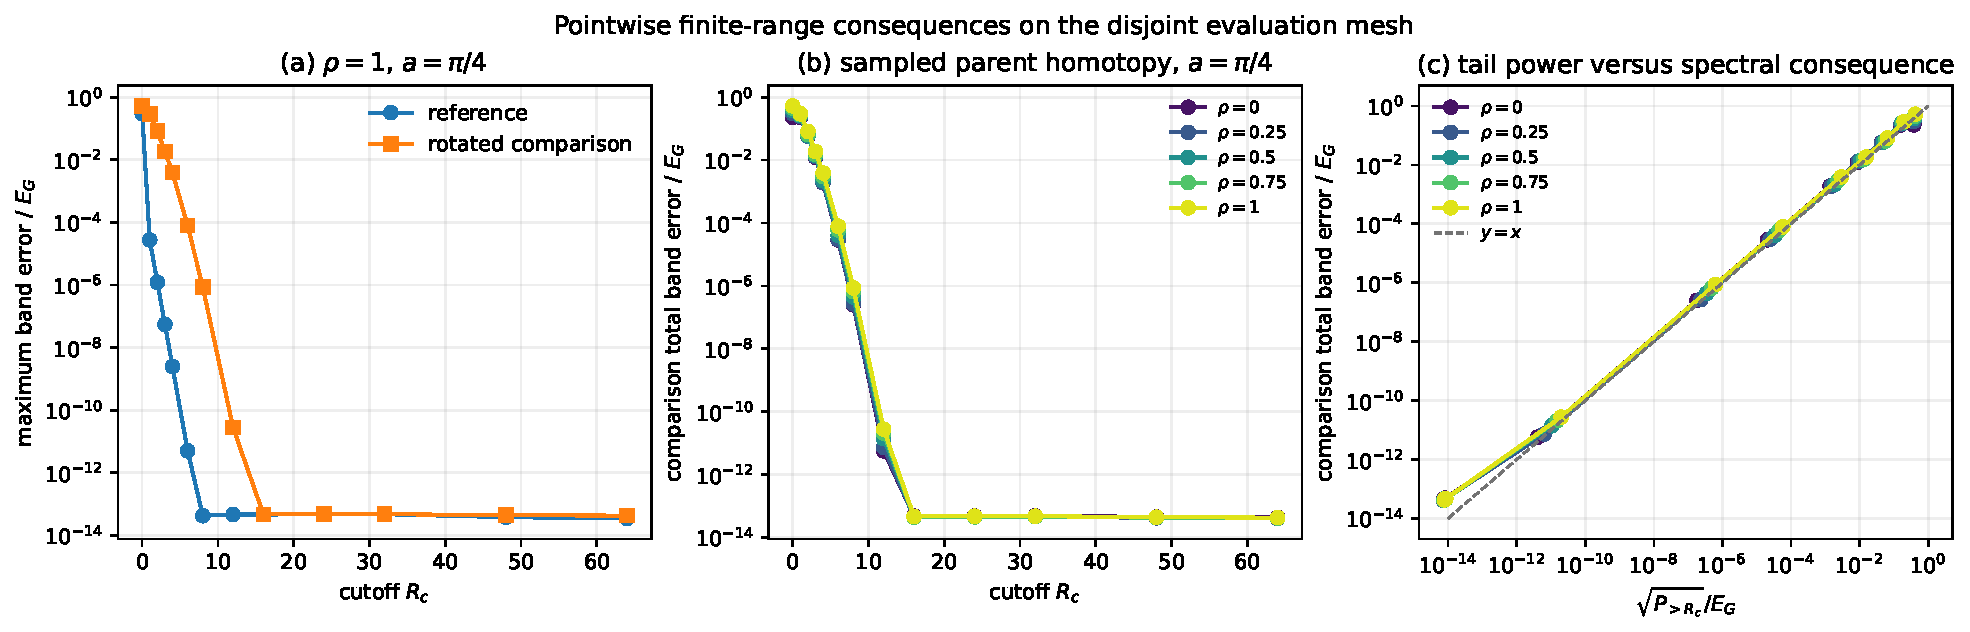
\includegraphics[width=\textwidth]
    {analysis/truncation-band-consequences.pdf}
  \caption{Pointwise finite-range consequences after explicit ordinary-lattice
  truncation. \textbf{(a)} Maximum reference and rotated-comparison band errors for the
  dispersive endpoint $(\rho,a)=(1,\pi/4)$. \textbf{(b)} Comparison total band error
  across the five sampled parent scales at $a=\pi/4$. \textbf{(c)} Comparison total band
  error against the square root of total omitted block power; the dashed $y=x$ line is a
  visual comparator, not an identity or bound. The centered cyclic Nyquist block is
  removed and reported separately before PhysKit applies each conjugate-closed cutoff.
  Lines connect directly calculated cutoffs as guides to the eye. The binary64 floor,
  finite $\rho$ and amplitude samples, and lack of a frozen accuracy target preclude a
  continuous range-to-accuracy certificate. This is pre-version development analysis,
  not retained evidence or material validation.}
  \label{fig:truncation-consequences}
\end{figure}

Across the sampled family, direct pointwise unitary comparison preserves the two bands
within $1.33\times10^{-15}E_G$, and the maximum full-comparison interpolation defect on
the disjoint mesh is $2.40\times10^{-14}E_G$. At $(\rho,a)=(1,\pi/4)$, $R_c=3$ gives a
reference maximum band error of $5.53\times10^{-8}E_G$ but a comparison total band error
of $1.86\times10^{-2}E_G$. At $R_c=8$, those values are
$4.22\times10^{-14}E_G$ and $8.65\times10^{-7}E_G$, respectively
[Fig.~\ref{fig:truncation-consequences}(a)]. The same qualitative ordering persists
through the five sampled parent scales [Fig.~\ref{fig:truncation-consequences}(b)]. Thus,
at the sampled nodes, complete band-equivalent Hamiltonians can require substantially
different finite hopping ranges for comparable band accuracy.

Figure~\ref{fig:truncation-consequences}(c) shows that square-root omitted power and
maximum band error track closely in this synthetic inventory, but no equality, upper
bound, or universal range-to-accuracy law is inferred. The action does not report
velocity, curvature, or physical effective mass. Its cutoff targets, independent result
verification, strict serializer, and retained-evidence contract remain prospective.

\section{Numerical-resolution study}

\subsection{Nested construction meshes}

The proposed construction meshes are
\begin{equation}
 N\in\{32,64,128,256,512\},
 \qquad
 q_i=-\frac12+\frac{i}{N},
 \quad i=0,\ldots,N-1.
 \label{eq:construction-meshes}
\end{equation}
Here $N$ is the number of momentum samples in one reciprocal-space quadrature, not the
number of independent model calculations. For example, $N=64$ means that the single
matrix-valued function $K(q)$ is assembled and diagonalized at 64 distinct momenta. The
matrices differ because the phase $e^{2\pi iqR}$ differs at each momentum. No parent
parameter is refitted between points.

The momentum grids are nested under doubling: every point on an $N$-point grid is an
even-index point on the $2N$-point grid. Previously evaluated points may therefore be
reused, and a complete refinement through $N=512$ contains 512 unique construction
momenta rather than the sum of all mesh sizes.

The completed flat-parent convergence study uses one fixed set of 65 amplitudes at every
momentum resolution. Its `converged' disposition concerns momentum refinement only. It
compares finite-mesh maximum correlation, the two thresholds, non-onsite hopping weight,
shared-block Fourier power, maximizing-angle status, the finite-mesh--Bessel quadrature
defect, band defect, the three-way identity defect, and Parseval defect. The discrete
$\mu_{N,\max}(a)$ and analytic $J_0(2a)$ remain separate. The amplitude interpolation
study in Fig.~\ref{fig:flat-parent-analysis}(b) is an additional analysis and is not part
of that momentum-convergence disposition.

The initial non-flat convergence implementation compares the sampled external gap,
shared-node parent eigenvalues and retained spectral projectors, frame orthonormality and
closure, Hermiticity, harmonic maximum and maximizing-angle status, $\mu_{N,\max}$, the
two thresholds, Fourier-block powers, non-onsite weight, band defect, quadratic
reconstruction, and Parseval consistency. The neighboring-frame transport singular
value is a per-mesh rank-qualification lower bound, not a convergence observable. The
study has no $J_0(2a)$ analytic comparator and may not assume the flat-parent three-way
locality identity. Full parent eigenvalue and projector arrays, admissible-set
quadratics, rectangle minima, witness coordinates,
support points, containment margins, separation bounds, and post-decision evaluation
losses remain prospective extensions. Its amplitude refinement must use a reviewed
direct or adaptive rule that replaces the inadequate proposed ladder in
Eq.~\eqref{eq:amplitude-mesh}.

For a scalar, vector, or matrix quantity $z$, the proposed continuous convergence test is
\begin{equation}
 \norm{z_{\mathrm{fine}}-z_{\mathrm{coarse}}}_\infty
 \le
 \epsilon_{\mathrm{abs}}
 +\epsilon_{\mathrm{rel}}
  \max\!\left(1,\norm{z_{\mathrm{fine}}}_\infty\right),
 \label{eq:convergence-test}
\end{equation}
with draft values
$\epsilon_{\mathrm{abs}}=10^{-10}$ and
$\epsilon_{\mathrm{rel}}=10^{-8}$. These are deterministic numerical tolerances, not
physical error bars or probabilistic confidence limits.

For the completed flat-parent momentum study, every implemented continuous channel must
pass on two successive refinements and maximizing-angle status must remain unchanged on
the corresponding three levels. For a final non-flat study, every continuous
quantity must pass on two successive refinements, every discrete disposition must remain
unchanged on three successive levels, and every decisive threshold or separation margin
must be at least ten times larger than the corresponding observed refinement change. If
the applicable momentum or amplitude cap is reached first, qualification fails. The
largest attempted mesh is not called converged merely because no larger calculation was
performed.

\subsection{Disjoint post-decision evaluation}

After the construction size $N_*$ has been selected, the evaluation mesh has size
\begin{equation}
 M=4N_*+1
 \label{eq:evaluation-size}
\end{equation}
and coordinates
\begin{equation}
 \widetilde q_\ell=-\frac12+
 \frac{\ell+1/(N_*+1)}{M},
 \qquad \ell=0,\ldots,M-1.
 \label{eq:evaluation-mesh}
\end{equation}
The rational offset makes these coordinates distinct from the construction coordinates.
A future retained implementation must additionally check all coordinate separations in
the physical reciprocal unit against a fixed tolerance.

For the full non-flat workflow, the disposition, witness, alignment, and
separation certificate are fixed before the evaluation mesh is examined. Reference and
comparison matrices at evaluation coordinates are reconstructed from the finite Fourier
representation obtained on the construction mesh. The selected candidate is then
evaluated without refitting. This procedure probes interpolation and aliasing behavior
between construction nodes. It does not create statistical independence, estimate
experimental uncertainty, or validate the parent model. Neither current smooth implementation assigns a post-decision admissible-set disposition
or executes this evaluation-mesh workflow. The exploratory finite-range consequence
action defined below does execute the disjoint mesh, but it does not issue an
admissible-set disposition or retained evidence.

\section{Fourier reconstruction and locality}

For the selected construction mesh, the matrix-valued forward transform is
\begin{equation}
 T_R^{(N_*)}=\frac{1}{N_*}\sum_{i=0}^{N_*-1}
 e^{-2\pi iq_iR}H(q_i),
 \label{eq:forward-fourier}
\end{equation}
and the finite trigonometric interpolant is
\begin{equation}
 H_{N_*}(q)=\sum_R e^{+2\pi iqR}T_R^{(N_*)}.
 \label{eq:inverse-fourier}
\end{equation}
The identity $H_{N_*}(q_i)=H(q_i)$ holds at the construction nodes. Away from those
nodes, $H_{N_*}$ is a finite interpolant and is not substituted for the continuous field
without an explicit interpolation or convergence check. The displacement inventory uses
centered integer representatives of the finite cyclic mesh. For an even mesh, the
Nyquist representative is $-N_*/2$; Hermitian symmetry there is interpreted cyclically,
so its block must be Hermitian. The calculation and verifier must share this convention.

For maximum retained range $R_c$, the finite-mesh omitted-block locality norm is
\begin{equation}
 \eta_{N_*}(R_c)=
 \left[
 \sum_{|R|>R_c}\norm{T_R^{(N_*)}}_F^2
 \right]^{1/2}.
 \label{eq:locality}
\end{equation}
It is evaluated separately for the reference matrix, comparison matrix, and selected
aligned candidate. The reported value retains the parent energy unit. The calculation
checks Fourier reconstruction, Parseval consistency under the declared normalization,
and cyclic Hermitian hopping symmetry
$T_{(-R)\bmod N_*}^{(N_*)}=(T_R^{(N_*)})^\dagger$. Locality ranges are fixed before
execution, listed in increasing order, and kept strictly below half the construction
mesh.

These diagnostics describe the selected finite mesh and basis. They are not general
claims of exponential localization, compressibility, or material accuracy.

\section{Exploratory finite-range consequence layer}

The active development action converts an even finite-cyclic inventory to an ordinary
integer-lattice inventory before applying any range cutoff. It removes the single
centered Nyquist representative $-N_*/2$ rather than treating it as self-conjugate on
the ordinary lattice. Its separately reported conversion power is
\begin{equation}
 P_{\mathrm{Nyq}}=\frac{1}{2E_G^2}
 \left\|T_{-N_*/2}^{(N_*)}\right\|_F^2,
 \label{eq:nyquist-conversion-power}
\end{equation}
where the factor two is the retained-state rank. The remaining inventory
$\mathcal R_{\mathrm{ord}}=\{-N_*/2+1,\ldots,N_*/2-1\}$ must pass PhysKit's
ordinary-lattice test $T_{-R}=T_R^\dagger$. This conversion channel is not silently
combined with deliberate range truncation.

For every prospectively declared integer $0\le R_c<N_*/2$, KSD passes the explicit
conjugate-closed set $\{-R_c,\ldots,R_c\}$ to PhysKit's
\texttt{ConjugateClosedBlockHoppingTruncator}. The resulting distinct model is
\begin{equation}
 H_{N_*,R_c}^{\mathrm{ord}}(q)=
 \sum_{|R|\le R_c}e^{2\pi iqR}T_R^{(N_*)}.
 \label{eq:ordinary-truncated-model}
\end{equation}
PhysKit reports raw omitted block power; KSD divides by $2E_G^2$ and reports both the
ordinary omitted power and its sum with Eq.~\eqref{eq:nyquist-conversion-power}.
Neither quantity is labeled a spectral error.

On the disjoint mesh of Eq.~\eqref{eq:evaluation-mesh}, let
$H_N^{\mathrm{ord}}$ and $A_N^{\mathrm{ord}}$ denote the untruncated ordinary-lattice
reference and comparison interpolants. Define the direct pointwise comparison
\begin{equation}
 A_{N,a}^{\mathrm{dir}}(q)=
 U_a(q)^\dagger H_N^{\mathrm{ord}}(q)U_a(q).
 \label{eq:direct-evaluation-comparison}
\end{equation}
Every ordinary model first passes the declared block-Hermiticity tolerance. Evaluated
Bloch matrices must also pass that tolerance; the sorted two-band spectrum is then taken
from the explicit Hermitian part $(H+H^\dagger)/2$ so that an eigensolver cannot silently
choose one triangle of a roundoff-level non-Hermitian matrix. The action reports maximum
and root-mean-square errors in three distinct channels:
\begin{align}
 \Delta_{\mathrm{interp}} &:
   \operatorname{eig}(A_N^{\mathrm{ord}})-
   \operatorname{eig}(A_{N,a}^{\mathrm{dir}}),\\
 \Delta_{\mathrm{trunc}} &:
   \operatorname{eig}(A_{N,R_c}^{\mathrm{ord}})-
   \operatorname{eig}(A_N^{\mathrm{ord}}),\\
 \Delta_{\mathrm{total}} &:
   \operatorname{eig}(A_{N,R_c}^{\mathrm{ord}})-
   \operatorname{eig}(A_{N,a}^{\mathrm{dir}}).
 \label{eq:truncation-error-channels}
\end{align}
The reference truncation channel is analogously compared with
$H_N^{\mathrm{ord}}$. Equation~\eqref{eq:truncation-error-channels} prevents finite-mesh
interpolation or aliasing error from being attributed to deliberate range deletion.
Here ``total'' means interpolation plus range truncation relative to the direct
ordinary-lattice field. No off-node Hermitian spectrum is assigned to the removed cyclic
Nyquist term; its conversion evidence remains the distinct power in
Eq.~\eqref{eq:nyquist-conversion-power}. Complete direct reference and comparison
matrices remain unitarily related before truncation.

This layer is exploratory: its cutoff inventory has not been frozen as a retained
protocol, strict non-flat serialization and independent result verification are not yet
implemented, and no range-to-accuracy acceptance threshold is issued. It reports only
band-energy consequences. Velocity, reduced-coordinate curvature, and physical
effective mass are excluded until derivative definitions, internal-band nondegeneracy,
$a_0$, $E_G$, and physical units have been reviewed.

\section{Independent verification and reproducibility}

\subsection{Current numerical owners}

The pre-version implementation consumes the exact revisions
\begin{center}
\small
\texttt{projectkoios-optimization}\\
\texttt{7ac5376bcb97e29f6927dda4d4ef714ed2e32140}\\[2pt]
\texttt{projectkoios-physkit}\\
\texttt{ed2e8118db9902316797d270305456735fab9712}.
\end{center}
Optimization owns continuous harmonic maximization and each complex-unitary pairwise
Procrustes solve in the producer. A numerically deficient overlap returns singular and
rank evidence but no full unitary transformation; KSD then applies the stricter declared
transport-overlap qualification gate. PhysKit owns immutable matrix-valued hopping
records, raw block Frobenius powers, and unit-aware complete bands from block-hopping
Bloch evaluations. PhysKit's band actions consume the canonical Numerics multi-series Fourier and batched
Hermitian-spectrum solvers and retain the correlated Bloch matrices, spectra, numerical
diagnostics, and backend evidence. The finite-range consequence action calls PhysKit's
ordered range-family evaluator so each source and its 13 retained models share one
reciprocal-grid phase matrix and one concatenated complete-spectrum solve. KSD supplies the finite-mesh identities, divides raw
powers by the retained rank and $E_G^2$, checks Parseval consistency, and interprets the
resulting locality and band-error channels.

PhysKit's hopping contracts use ordinary integer-lattice displacement semantics. The
complete even-$N$ Fourier inventory in this experiment remains cyclic and aliased: the
centered Nyquist representative $-N/2$ is self-conjugate only modulo $N$. KSD therefore
retains the cyclic Hermiticity check for the complete finite inventory. Any later
ordinary-lattice truncation must use a conjugate-closed retained set with
$R_c<N/2$, excluding the Nyquist representative. No owner API converts the finite
coefficients into continuous hoppings without a convergence argument.

\subsection{Independent numerical reconstruction}

The implemented flat-parent verifier reads canonical input and result records but does
not call the producing experiment action or trust a serialized disposition. It
independently reconstructs the sampled matrices, band defect, second-harmonic
coefficients, continuous maximum and unique-or-degenerate angle status, finite-mesh and
analytic correlations, thresholds, Fourier-block powers, non-onsite weight, Parseval
identity, and flat-parent three-way identity. Its convergence verifier separately
reconstructs every adjacent momentum-mesh comparison and the final `converged' or
`unresolved' disposition.

The implemented `SmoothFourStateVerifier' independently reconstructs
Eq.~\eqref{eq:parent-bloch}, repeats the eigensystem and frame checks, reconstructs the
comparison field, Fourier blocks, Parseval quantities, and original restricted-alignment
loss, and obtains the harmonic maximum directly as
$b_0+\sqrt{c^2+d^2}$ without calling the producer's Optimization maximizer. A future
full verifier must additionally rebuild $Q$, $g$, and $c$ from
Eq.~\eqref{eq:quadratic}; recompute rectangle minima; check witness membership; derive
support points through linear solves; verify containment; reconstruct lower and upper
separation bounds; and apply
Eqs.~\eqref{eq:forward-fourier}--\eqref{eq:locality} to disjoint evaluation channels.
Those prospective certificate checks are not claimed as current four-state coverage.

Verification reports contain channel-resolved maximum defects rather than only a Boolean
pass flag. Dimensionless defects and energy-valued defects remain separate. The main
calculation and verifier may share binary64 arithmetic and the same numerical library;
that dependence is disclosed. Independence here means separate scientific
reconstruction and control flow, not independent hardware or an unrelated eigensolver.

\subsection{Serialization and evidence}

The implemented flat-parent input, result, and verification records use strict JSON
schemas that reject unknown fields. Non-flat schemas are intentionally deferred until
its numerical contract is reviewed. Numeric strings and Boolean values presented as real
numbers are rejected by the applicable public contracts.
Floating-point values must be finite. Complex values are represented by explicit real
and imaginary components, and arrays carry fixed dimensions wherever shape is part of
the scientific contract.

The active result records the SHA-256 digest of the exact canonical input bytes. The
verification record binds both input and result digests. Family, schema, and method
identities are checked against expected values rather than trusted from the payload, and
the input scope explicitly states that the calculation is not retained. Any change to a
nested value or immutable identity either changes the digest or fails schema validation.
A future retained schema must additionally bind immutable version and run identities;
no such identity is inferred for the current pre-version records.

A retained run directory will be created by an exclusive no-overwrite operation. It will
contain canonical input, result, and verification records; the complete convergence table;
source and dependency provenance; platform and command information; authenticated
schema identities; the exact source manifest; a checksum manifest; and a readable
report separating controls, calculated quantities, and interpretation. Experiment
version, run identity, and content-addressed evidence-package identity remain distinct.

\subsection{Failure policy}

The active flat-parent calculation fails closed on nonfinite data, invalid dimensions,
malformed amplitudes or reciprocal meshes, nonpositive convergence thresholds, failed
harmonic reconstruction, failed Fourier or Parseval identities, schema violations,
digest mismatch, or disagreement with the verifier. The initial non-flat calculation
additionally fails closed on inadequate external gap, rank-deficient transport, failed
frame closure, inconsistent loss reconstruction, failed Fourier nodal reconstruction,
Parseval inconsistency, or disagreement with its verifier. The future expanded contract
must also fail closed on nonpositive raw weights, malformed or reused evaluation
coordinates, indefinite quadratics, invalid certificates, and checksum mismatch. Such
failures do not become scientific outcomes.

An empty admissible component, an invalid containment premise, an insufficient
separation margin, or failure to find a common witness can be a legitimate scientific
non-result. These conditions lead to an empty-component record, an invalid-premise
record, or an unresolved disposition rather than a software success being reinterpreted
as evidence.

\section{Prespecified controls and execution status}

Table~\ref{tab:controls} separates the mathematical design already stated in this
manuscript from controls that still require final scientific review. Confirmatory
execution is not permitted until every open control has a value, unit, rationale, and
canonical representation.

\begin{table}[htbp]
\centering
\caption{Status of outcome-relevant controls. ``Specified'' means that the value or rule
appears in this manuscript. ``To be fixed'' means that no confirmatory calculation may
proceed until the control is approved and recorded.}
\label{tab:controls}
\begin{tabular}{>{\raggedright\arraybackslash}p{0.39\textwidth}
                >{\raggedright\arraybackslash}p{0.20\textwidth}
                >{\raggedright\arraybackslash}p{0.31\textwidth}}
\toprule
Control & Status & Location or required record \\
\midrule
Parent hopping model and reciprocal convention & Specified &
Eqs.~\eqref{eq:parent-bloch} and preceding matrices \\
Retained rank and frame method & Specified &
Eqs.~\eqref{eq:parallel-transport}--\eqref{eq:closure-correction} \\
Minimum external gap & To be fixed & Positive energy-valued lower bound and rationale \\
Minimum transport-overlap singular value & Draft value only &
Final $\sigma_{\mathrm{rank}}$ and tolerance \\
Comparison rotation field & Specified & Smooth family in
Eq.~\eqref{eq:attacked-matrix} \\
Candidate and continuous alignment families & Specified &
Eqs.~\eqref{eq:candidate}--\eqref{eq:continuous-maximizing-angle} \\
Momentum construction and evaluation rules & Specified &
Eqs.~\eqref{eq:construction-meshes}--\eqref{eq:evaluation-mesh} \\
Amplitude refinement rule & To be fixed & Direct analytic or reviewed adaptive rule \\
Parameter rectangle & To be fixed & Four dimensionless bounds \\
Spectral and operator thresholds & To be fixed & Values, units, and scientific status \\
Separation resolution & To be fixed & $\rho_{\mathrm{sep}}$ and its rationale \\
Locality ranges & To be fixed & Ordered integer ranges \\
Numerical tolerances & Draft values only & Channel-specific finalized table \\
Software revisions & Development known; retained open &
Dependency lockfiles; exact retained manifests \\
Confirmatory execution authorization & Not granted & Separate operator decision \\
\bottomrule
\end{tabular}
\end{table}

\section{Interpretation and limitations}

Theorem~\ref{thm:exact-loss-geometry} is not specific to the numerical parent matrices.
It applies to any sampled rank-two Hermitian field with positive weights, a comparison
target related by unitary conjugation, and the trace--traceless candidate family in
Eq.~\eqref{eq:candidate}. The parent, momentum dependence, and continuous global
alignment enter the optimized geometry through $\kappa$ and $\mu_{\max}$.

An instance-specific conclusion applies only to the stated parent model, retained
rank-two subspace, frame convention, comparison representation, candidate family,
parameter rectangle, continuous global real-rotation family, thresholds, numerical
resolution, and data roles.
A compatible result would show that one parameter pair meets the two declared limits in
this controlled setting. A separated result would show that the two admissible regions
are farther apart than the declared resolution under the verified geometric premises.
Neither result would establish material validity, parent-model correctness, uncertainty
quantification, uniqueness, continuum convergence, or adequacy under unrestricted
momentum-dependent unitaries.

The frame, matrix loss, and locality norms are basis dependent by design. The spectral
loss is basis invariant. If the full generating $U_a(q)$ is accepted as the state-space
identification, $H(q)$ and $A_a(q)$ are unitarily equivalent representations and their
abstract-operator difference is zero. The reported nonzero residual instead answers the
declared restricted question in which only one momentum-independent real rotation may
identify retained coordinates. Keeping these channels and identification rules separate
is essential to the scientific question rather than a technical inconvenience.
Likewise, convergence of the spectrum does not imply convergence of represented
matrices, hopping blocks, or geometric certificates; each applicable channel is
therefore tested explicitly.

No Quantum ESPRESSO or Wannier90 calculation is part of this controlled protocol. A
material application would require a separate authorized design specifying structures,
pseudopotentials, exchange--correlation approximation, cutoffs, meshes, Wannier
windows and projections, energy alignment, resource estimates, and provenance.

\bibliographystyle{unsrt}
\bibliography{experimental-protocol}

\appendix

\section{Exact rectangle minimization}

For
\[
 f(p)=(p-p_c)^TQ(p-p_c)+m,
 \qquad
 Q=
 \begin{pmatrix}Q_{11}&Q_{12}\\Q_{12}&Q_{22}\end{pmatrix},
\]
the unconstrained center is included when it lies in $X$. On a vertical edge $p_1=b$,
the unconstrained edge minimizer is
\[
 p_2=p_{c,2}-\frac{Q_{12}}{Q_{22}}(b-p_{c,1}),
\]
which is clipped to $[\lambda_{\min},\lambda_{\max}]$. This is done for
$b=s_{\min}$ and $b=s_{\max}$. On a horizontal edge $p_2=b$, the corresponding minimizer
is
\[
 p_1=p_{c,1}-\frac{Q_{12}}{Q_{11}}(b-p_{c,2}),
\]
clipped to $[s_{\min},s_{\max}]$. Direct evaluation of the original quadratic at these
points yields the exact rectangle minimum for a positive-definite two-dimensional
quadratic. Corners appear automatically when clipping reaches an endpoint.

\section{Support and containment checks}

For a general quadratic ellipse
\[
 \mathcal E=\{p:(p-p_c)^TQ(p-p_c)\le\beta\},
 \qquad Q\succ0,
\]
the support point and support value in direction $d\ne0$ are
\begin{align}
 p_+(d)&=p_c+
 \sqrt{\frac{\beta}{d^TQ^{-1}d}}Q^{-1}d,\\
 \max_{p\in\mathcal E}d^Tp
 &=d^Tp_c+\sqrt{\beta\,d^TQ^{-1}d}.
\end{align}
Coordinate extrema are obtained using $d=(1,0)^T$ and $d=(0,1)^T$ together with their
negatives. Containment requires all four extrema to remain within the corresponding box
bounds after accounting for the fixed containment tolerance. The support calculation
uses linear solves with $Q$ and never substitutes a box-clipped point into a formula for
the full ellipse. For the common curvature in
Theorem~\ref{thm:exact-loss-geometry}, these checks reduce to the semiaxes stated by
Eqs.~\eqref{eq:exact-spectral-loss} and \eqref{eq:exact-operator-loss}.

A candidate upper bound on the distance is computed from an explicitly feasible pair
$(p_s,p_o)$ as $\norm{p_s-p_o}_2$. A projected lower bound is accepted only after its
support points, component orientation, containment premise, and threshold membership
have been independently reconstructed. The inequalities
\[
 0\le\underline\delta\le\delta^*\le\overline\delta
\]
must hold within numerical tolerance. A violation indicates a calculation or premise
failure, not an unusual scientific result.

\section{Execution sequence}

The confirmatory calculation follows the sequence below without adaptive changes to the
scientific controls.

\begin{enumerate}[label=\arabic*.]
  \item Parse canonical input and reject unknown, malformed, nonfinite, or inconsistent
        fields.
  \item Construct $K(q)$ on every mesh in the declared refinement ladder.
  \item Diagonalize the parent, retain the lowest two states, and verify the external
        gap and retained projectors.
  \item Build and periodically close the transported frame; stop on deficient overlap.
  \item Construct $H(q)$ and the complete amplitude family $A_a(q)$ and retain all
        parent diagnostics.
  \item For every momentum and amplitude mesh, construct the spectral quadratic and the
        exact second-harmonic operator correlation from the original residuals.
  \item Maximize the continuous harmonic over its half-open fundamental interval,
        record unique or degenerate angle status, construct the optimized operator
        quadratic, and minimize both quadratics over the fixed parameter rectangle.
  \item Apply all continuous and discrete convergence gates. Stop with failed
        qualification if the declared caps are reached first.
  \item Freeze the selected construction resolution without changing thresholds or
        parameter bounds.
  \item Search for a common witness and verify it from the original residuals.
  \item If no witness is established, test every separation-certificate premise and
        construct conservative lower and upper bounds.
  \item Assign the disposition from construction data and the declared numerical
        uncertainty rules.
  \item Generate the disjoint evaluation mesh and compute evaluation losses without
        changing the disposition.
  \item Transform the reference, comparison, and selected candidate matrices to hopping
        blocks and calculate range-resolved locality norms.
  \item Serialize canonical evidence, perform independent reconstruction, validate
        schemas and digests, and retain the package only if all required checks pass.
\end{enumerate}

\end{document}
